
\section{Benutzerhandbuch}

\subsection{Projektauswahlfenster}
Das Programm startet mit einem Auswahlfenster für Projekte. Hier haben Sie die Möglichkeit zuletzt erstellte Projekte zu öffnen, andere existierende Projekte hinzuzufügen oder ein neues Projekt zu erstellen. 

\begin{figure}[h!]
	\centering
	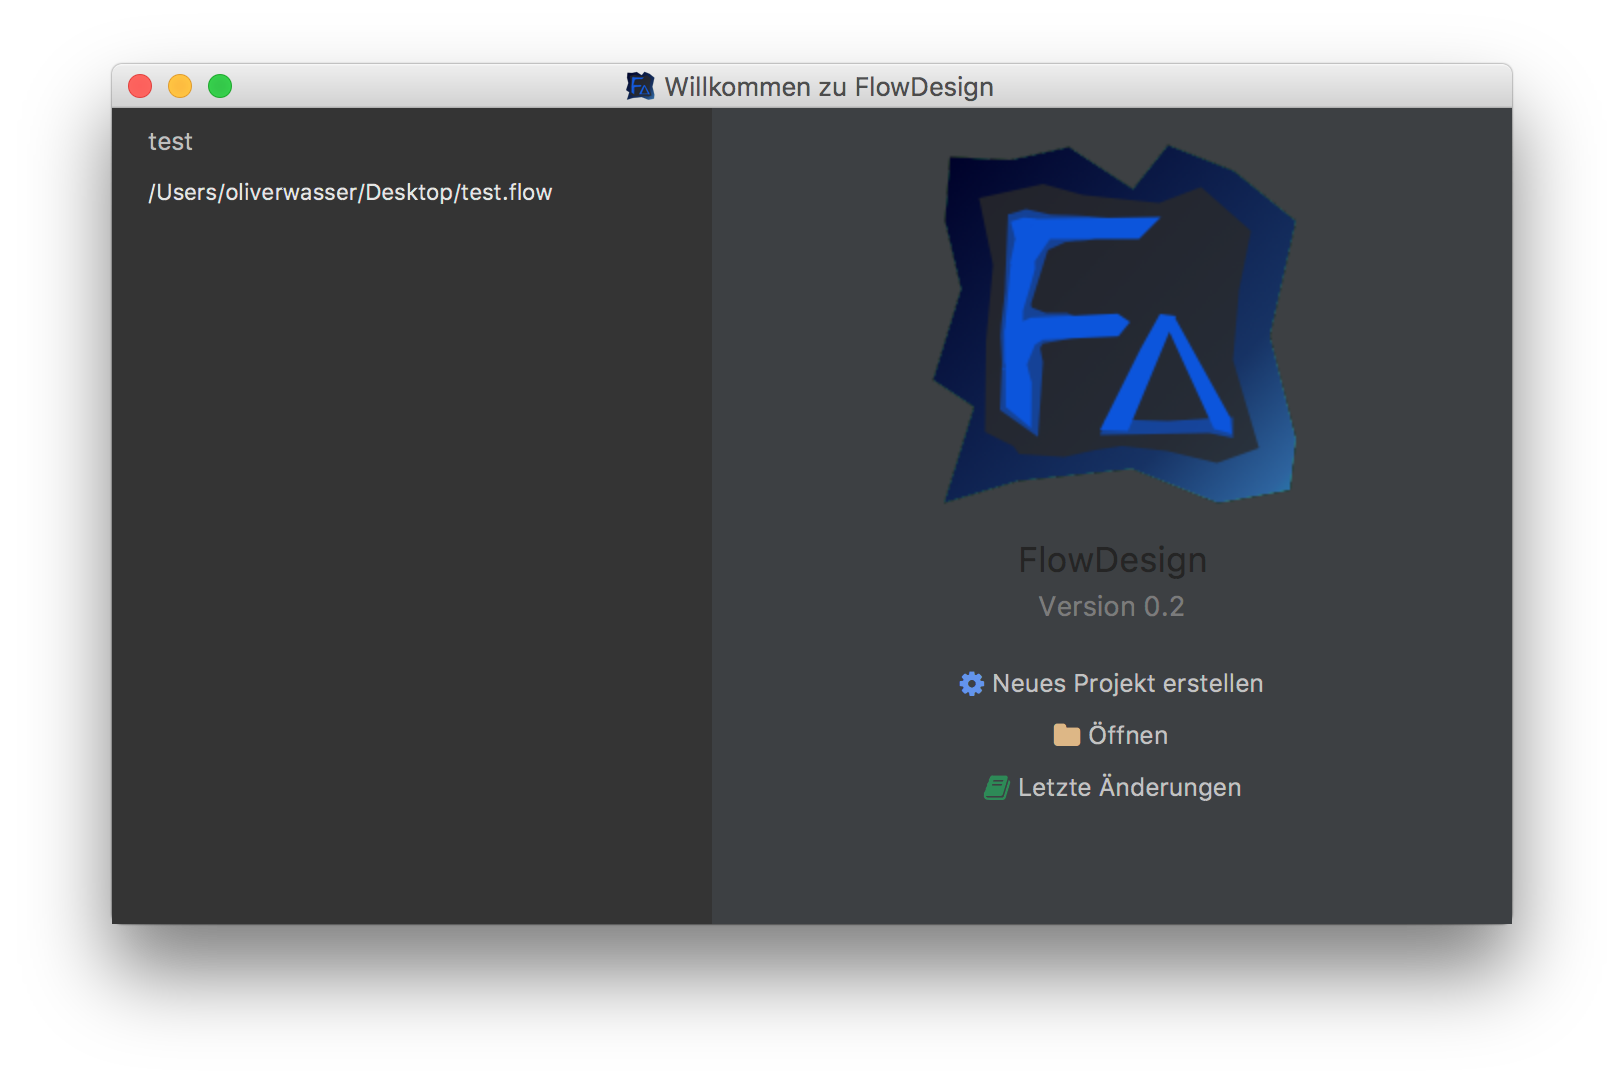
\includegraphics[width=1.0\textwidth]{Auswahlfenster.png}
	\caption{Auswahlfenster}
\end{figure}


\subsubsection{Öffnen eines kürzlich erstellten Projekts}
Zum Öffnen eines kürzlich erstellten Projekts, wählen Sie mit einem Doppelklick das gewünschte Projekt im linken Teil des Auswahlfensters.

\subsubsection{Öffnen eines beliebigen Projekts}
Zum Hinzufügen eines anderen bestehenden Projektes, wählen Sie mit einem Linksklick ''Öffnen''. Es erscheint ein Fenster zur Auswahl des Dateipfades. Wählen Sie nun das gewünschte Projekt als ''.flow'' Datei aus und bestätigen Sie anschließend.

\subsubsection{Erstellen eines neuen Projekts}
Zum Erstellen eines neuen Projektes, drücken Sie ''Neues Projekt erstellen''. Im folgenden Fenster tragen Sie einen Name und Speicherort für Ihr Projekt ein. Bestätigen Sie mit ''Ok''.


\subsection{Projektfenster}
\subsubsection{Menüleiste}
\begin{figure}[h!]
	\centering
	
\includegraphics[width=1.0\textwidth]{Leiste.png}
	\caption{Menüleiste unter macOS}
\end{figure}

\begin{figure}[h!]
	\centering
	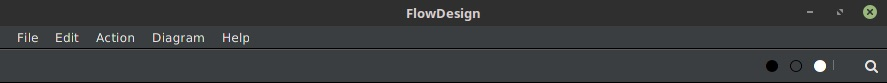
\includegraphics[width=1.0\textwidth]{Leiste2.jpg}
	\caption{Menüleiste unter Linux/Windows}
\end{figure}

Die Menüleiste enthält die Auswahlpunkte ''Datei'', ''Bearbeiten'', ''Aktion'', ''Diagramm'' und ''Hilfe''.
Die Sprache der Leiste wechselt automatisch zwischen Deutsch und Englisch, je nachdem unter welcher Sprache Ihr Betriebssystem eingestellt ist.
Die für die einzelnen Aktionen nötigen Shortcuts werden Ihnen jeweils zugehörig in der Menüleiste angezeigt. 




\begin{figure}[h!]
	\centering
	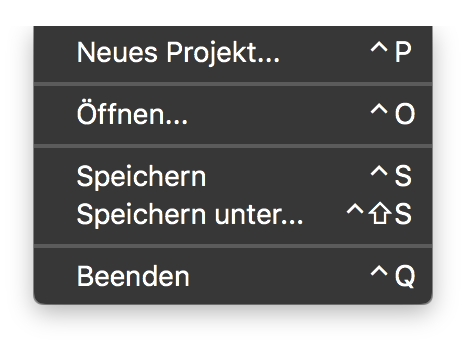
\includegraphics[width=.4\textwidth]{Leiste_Datei.png}
	\caption{Menüleiste - ''Datei''}
\end{figure}
Unter ''Datei'' ist es Ihnen möglich ein anderes Projekt zu öffnen, das aktuelle Projekt zu speichern oder mit ''Speichern unter'' eine neue Kopie unter einem beliebigen Pfad abzulegen.


\begin{figure}[H]
	\centering
	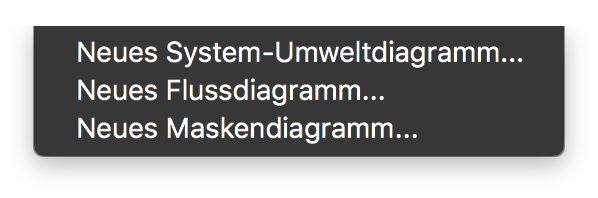
\includegraphics[width=.4\textwidth]{Leiste_Bearbeiten.png}
	\caption{Menüleiste - ''Bearbeiten''}
\end{figure}
Unter ''Bearbeiten'' haben Sie die Möglichkeit neue Diagramme jedes Typen zu erstellen.


\begin{figure}[H]
	\centering
	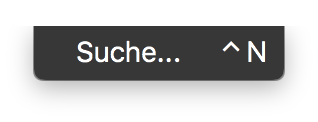
\includegraphics[width=.4\textwidth]{Leiste_Aktion.png}
	\caption{Menüleiste - ''Aktion''}
\end{figure}
''Aktion'' enthält die Suche nach Diagramme. Diese kann ebenfalls mit dem Lupensymbol in der oberen rechten Ecke des Programmes abgerufen werden.



\begin{figure}[H]
	\centering
	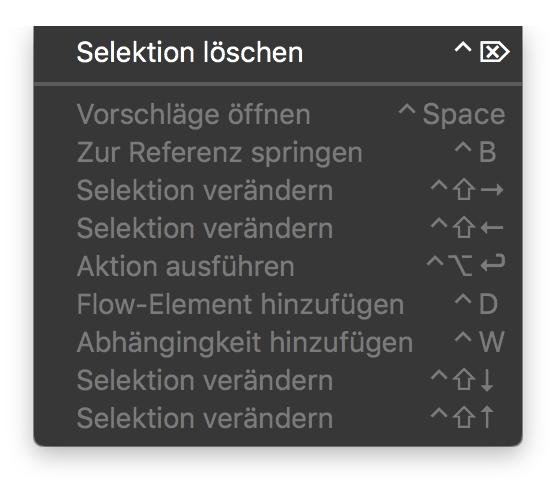
\includegraphics[width=.4\textwidth]{Leiste_Diagram.png}
	\caption{Menüleiste - ''Diagram''}
\end{figure}
Unter ''Diagramm'' finden Sie sämtliche Optionen die das intelligente Arbeiten mit Diagrammen betrifft. Dazu gehört der Quick-Jump in verlinkte Diagramme oder das Hinzufügen von Abhängigkeiten.



\begin{figure}[H]
	\centering
	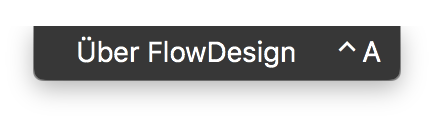
\includegraphics[width=.4\textwidth]{Leiste_Hilfe.png}
	\caption{Menüleiste - ''Hilfe''}
\end{figure}
Wählen Sie ''Hilfe'', um Informationen über den aktuellen Programmbuild zu erhalten.	






\begin{figure}[H]
\subsubsection{Projektbaum und Anlegen neuer Diagramme}
	\centering
	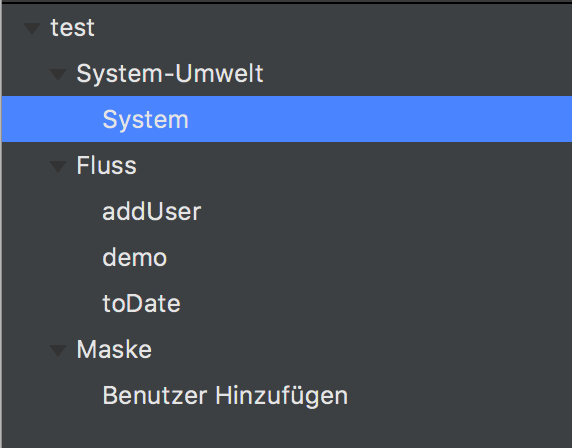
\includegraphics[width=.4\textwidth]{Projektbaum.png}
	\caption{Projektbaum}
\end{figure}
Der Projektbaum befindet sich im Programm auf der linken Seite.
In der obersten Zeile finden Sie Ihren zuvor gewählten Projektnamen wieder, gefolgt von den drei Diagrammtypen 'System-Umwelt', ‘Fluss‘ und ‘Maske‘. Sie können beliebig viele Diagramme eines Typs erstellen.


\begin{figure}[H]
	\centering
	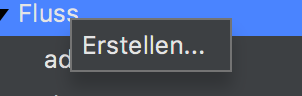
\includegraphics[width=.4\textwidth]{Projektbaum_Erstellen.png}
	\caption{Projektbaum - Erstellen}
\end{figure}
Um ein neues Diagramm zu erstellen, drücken Sie mit der rechten Maustaste auf den gewünschten Diagrammtyp. Wählen Sie nun ‘Erstellen' und vergeben Sie einen Namen, beachten Sie dabei das ein Name nur einmalig vergeben werden kann. 



\begin{figure}[H]
	\centering
	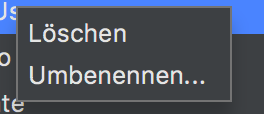
\includegraphics[width=.4\textwidth]{Projektbaum_Bearbeiten.png}
	\caption{Projektbaum - Bearbeiten}
\end{figure}
Um bereits erstellte Diagramme zu löschen oder umzubenennen, drücken Sie mit der rechten Maustaste auf das gewünschte Diagramm und wählen Sie die Änderung welche Sie vornehmen möchten. Wenn Sie ein Diagramm umbenennen, wird die Namensänderung durch das Programm automatisch in allen anderen Diagrammen und Referenzen übernommen.


\begin{figure}[H]
\subsubsection{Datentypen bearbeiten}
	\centering
	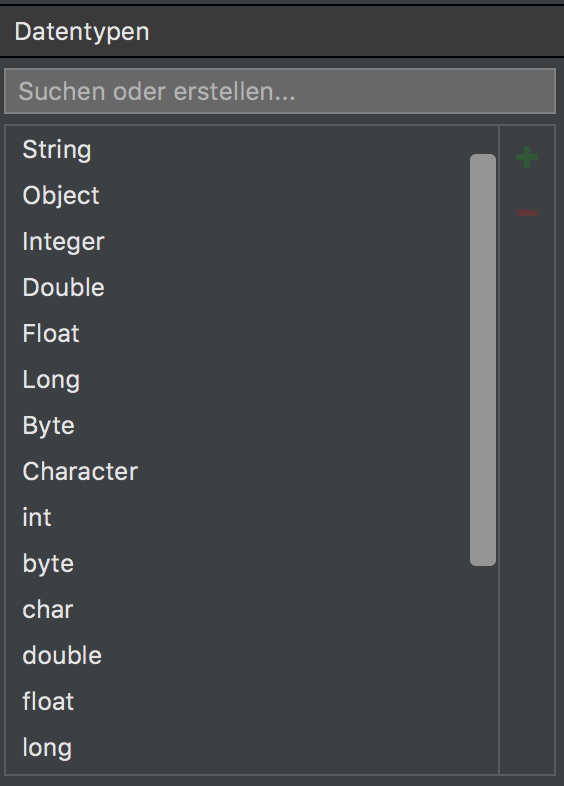
\includegraphics[width=.4\textwidth]{Datentypen.png}
	\caption{Datentypenliste}
\end{figure}
Sie können im linken Teil des Programmfensters eigene und bestehende Datentypen anlegen oder löschen. Diese werden alle in den einzelnen Diagrammen referenziert und können dort, etwa in der Autovervollständigung, genutzt werden.

\begin{figure}[H]
	\centering
	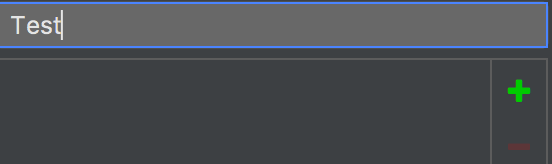
\includegraphics[width=.4\textwidth]{Datentypen_Add.png}
	\caption{Datentypenliste - Hinzufügen}
\end{figure}
Um einen neuen Datentyp hinzuzufügen, geben Sie den gewünschten Namen im Textfeld ein. Existiert bereits ein Datentyp mit dem Namen, wird es Ihnen in der Liste angezeigt. Zum Hinzufügen betätigen Sie nun das grüne Plus-Symbol. Der neue Datentyp erscheint nun in der Liste.

\begin{figure}[H]
	\centering
	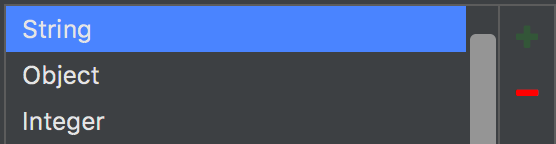
\includegraphics[width=.4\textwidth]{Datentypen_Delete.png}
	\caption{Zeichenfläche - Entfernen}
\end{figure}
Um einen Datentypen zu entfernen, markieren Sie diesen in der Liste mit einem Linksklick. Anschließend betätigen Sie das rote Minus-Symbol. Der Datentyp verschwindet nun aus der Liste. Datentypen, welche bereits in Diagrammen verwendet wurden, werden aus diesen nicht entfernt.




\begin{figure}[H]
\subsection{Zeichenfläche}
	\centering
	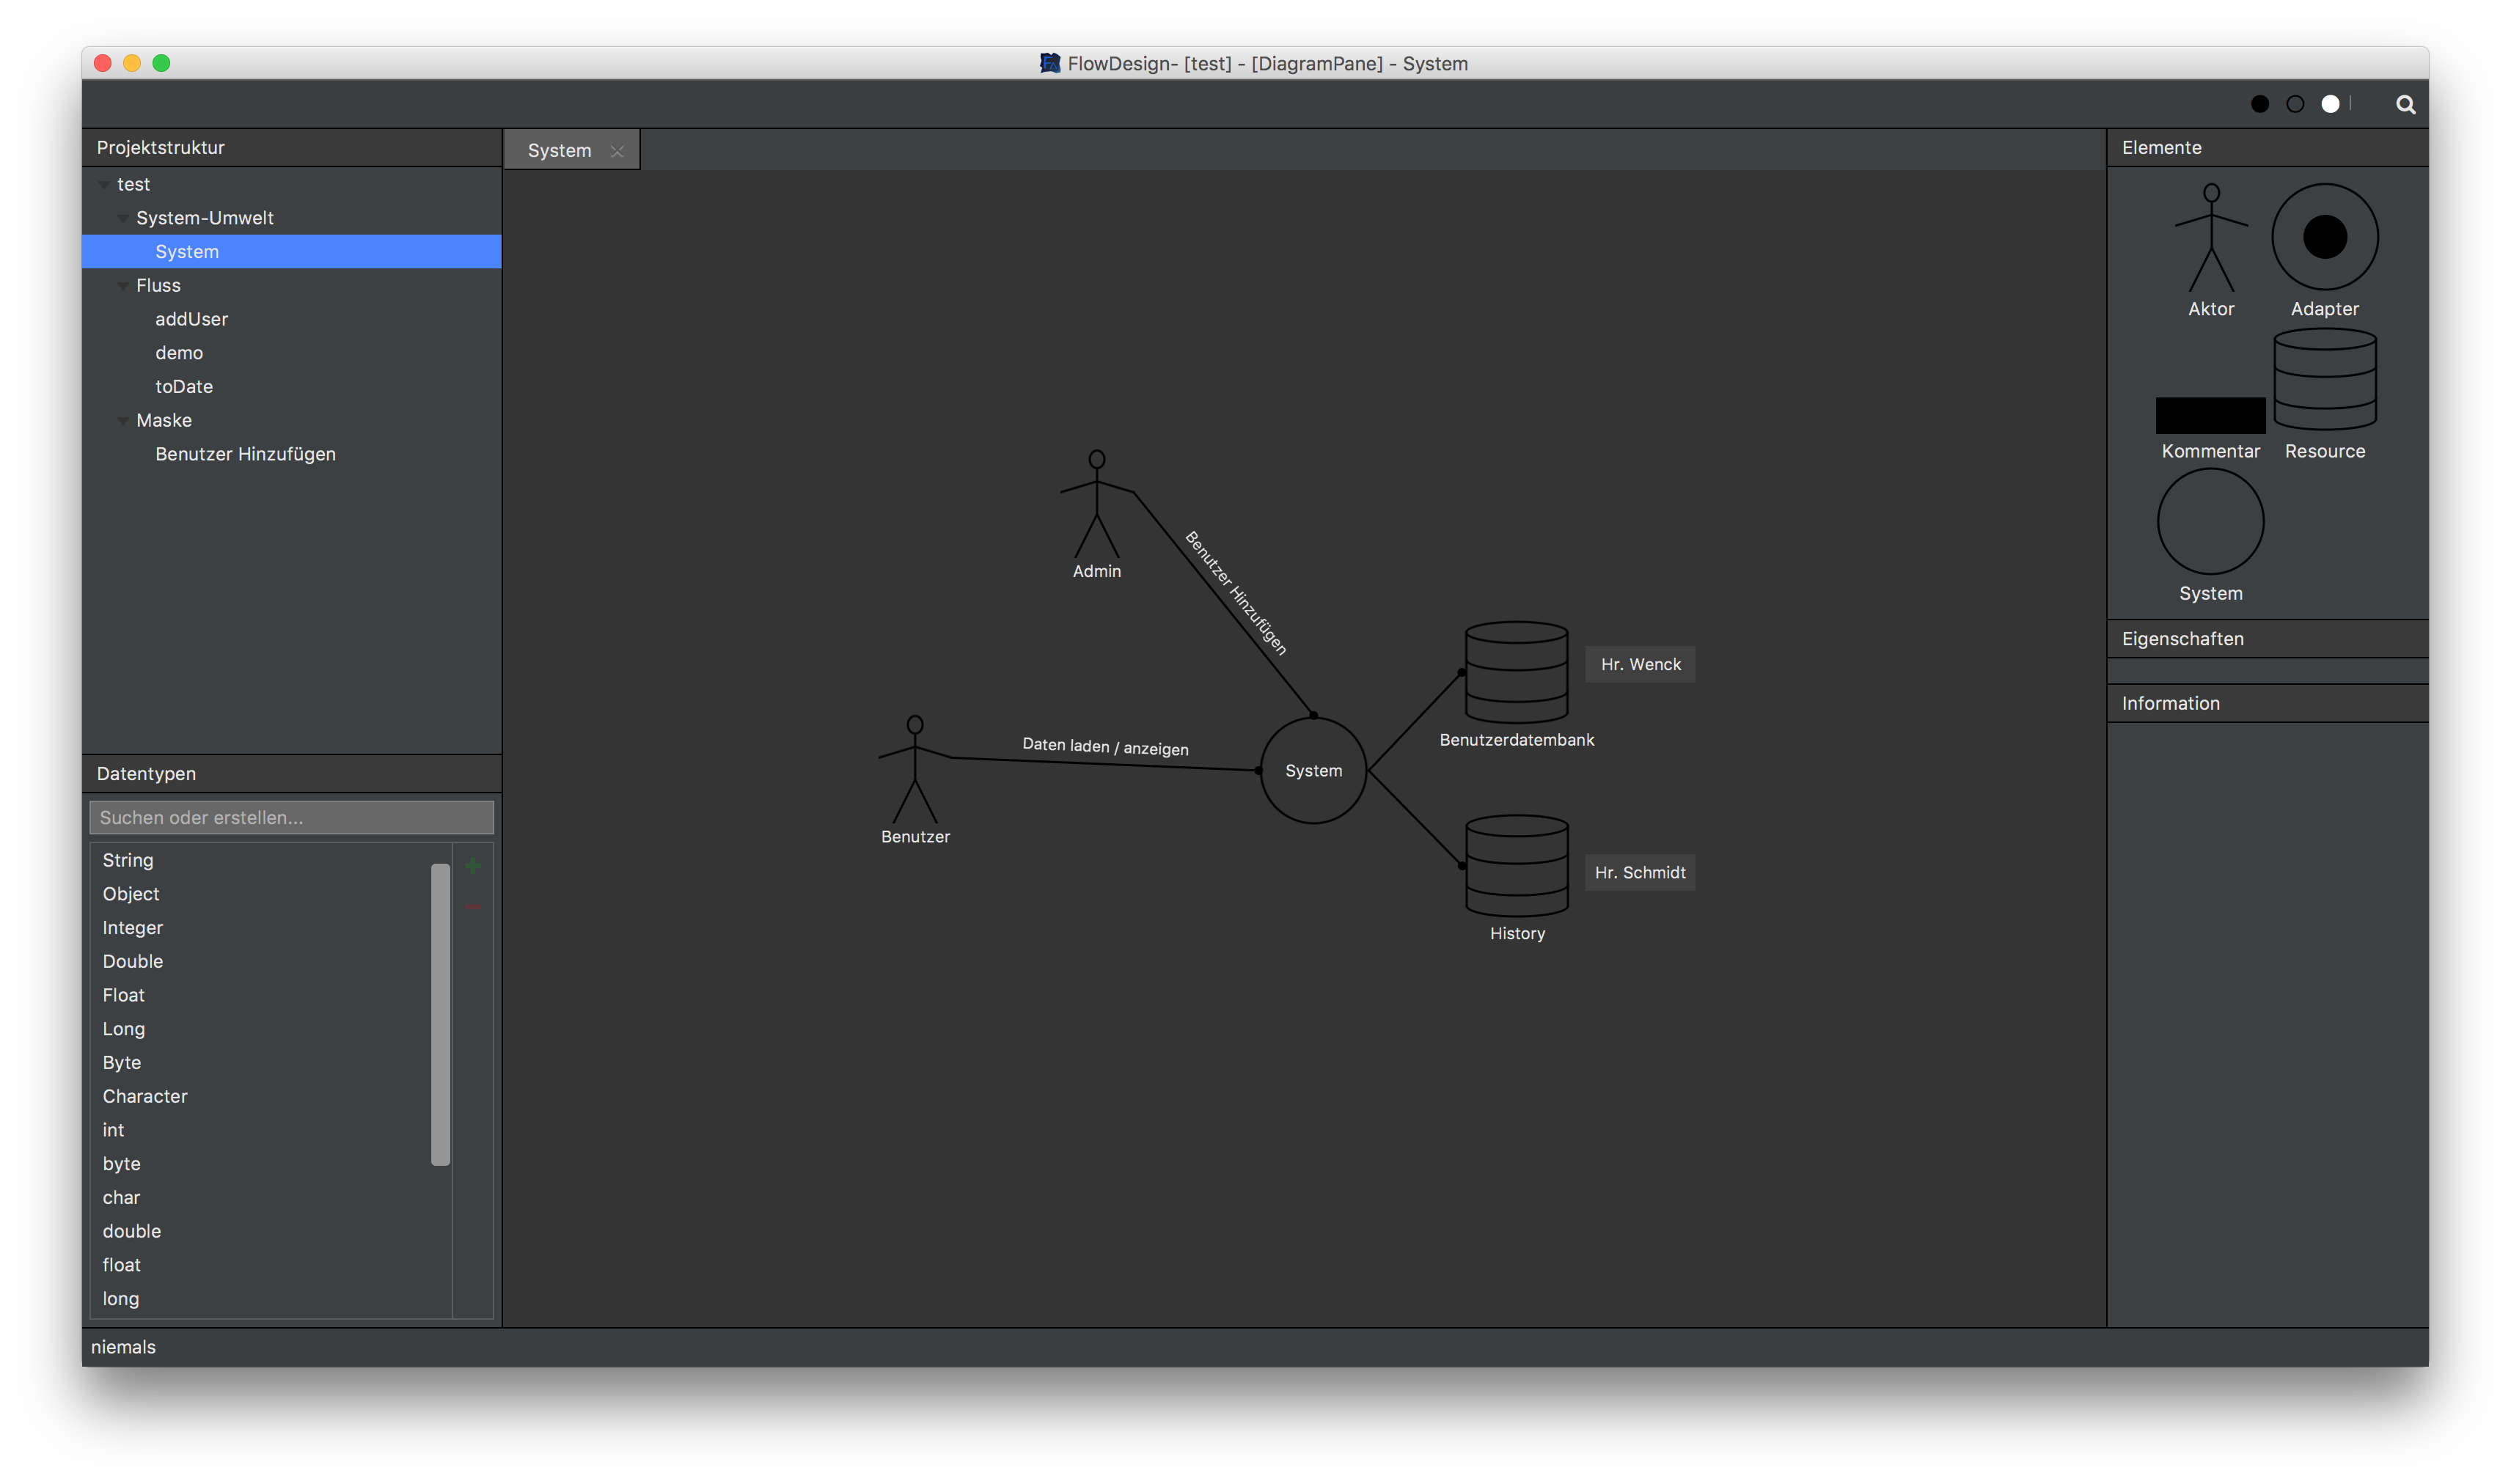
\includegraphics[width=1\textwidth]{Design_Dark.png}
	\caption{Zeichenfläche}	
\end{figure}
Bei der Zeichenfläche handelt es sich um das Oberflächenelement zum Bearbeiten von Diagrammen. 

\begin{figure}[H]
	\centering
	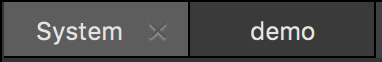
\includegraphics[width=.4\textwidth]{Tabs.png}
	\caption{Zeichenfläche - Tabs}	
\end{figure}
Im oberen Randbereich befinden sich Tabs von geöffneten Diagrammen. Um zwischen Tabs zu wechseln, wählen Sie mit einem Linksklick oben den gewünschten Tab aus.

\begin{figure}[H]
	\centering
	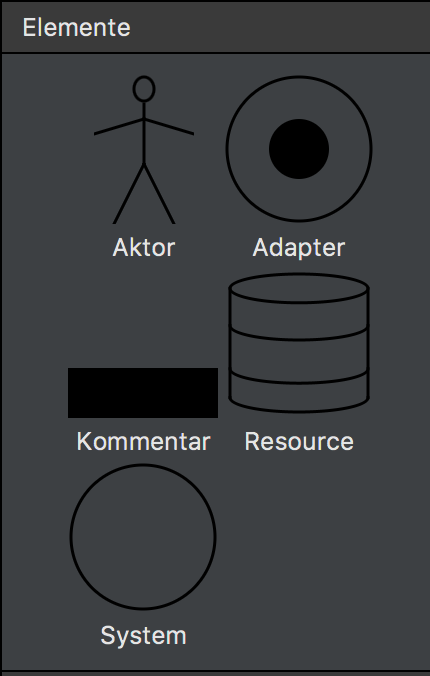
\includegraphics[width=.4\textwidth]{Elemente.png}
	\caption{Zeichenfläche - Elemente}	
\end{figure}
Rechts befindet sich eine Übersicht aller Elemente. Diese ändern sich je nach dem, in welchem Diagrammtyp man sich momentan befindet. Um ein Element hinzuzufügen, ziehen Sie dieses mit gedrückter Maustaste in das Zeichenfeld. 

\pagebreak
\begin{figure}[H]
	\centering
	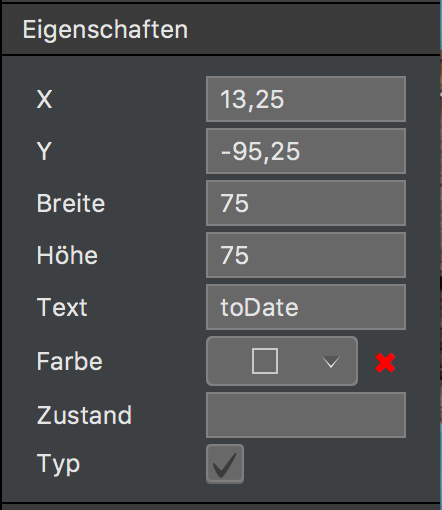
\includegraphics[width=.4\textwidth]{Eigenschaften.png}
	\caption{Zeichenfläche - Eigenschaften}
\end{figure}
Unter der Element-Auswahl befinden sich die Eigenschaften eines Elements. Um die Eigenschaften eines Elements zu verändern, markieren Sie es mit einem Linksklick. Je nach dem welches Element gewählt wurde, passen sich die dargestellten Eigenschaften automatisch an. Bei ''Zustand'' und ''Typ'' handelt es sich um spezielle Eigenschaften des Elements ''Operation''. Sollte eine Operation auf einen globalen Zustand des zu modellierenden Systems zugreifen, kann durch ''Zustand'' dessen Name angegeben werden. Mit ''Typ'' kann zwischen einem Ressourcenzugriff und einem Zustandszugriff unterschieden werden. Dabei ändert sich auch das angezeigte Icon der Operation. Eine weitere Besonderheit ist die Eigenschaft ''Portal'' im Flussdiagramm. Damit ist es möglich den Start/Ende durch Portale zu ersetzten.

\begin{figure}[H]
\subsubsection{Erstellen von Verbindungen}
	\centering
	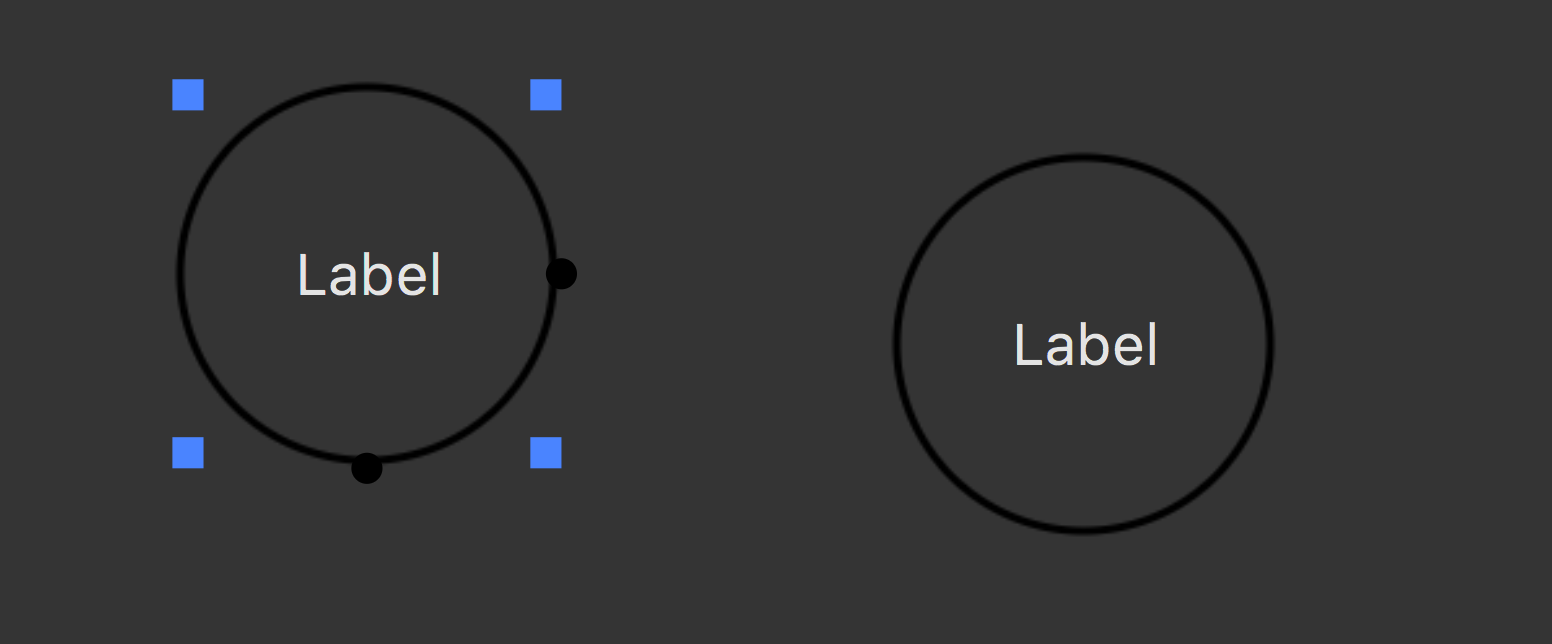
\includegraphics[width=.4\textwidth]{Zeichenflaeche_Basics.png}
	\caption{Zeichenfläche - Erstellen einer Verbindung}	
\end{figure}
Um eine Verbindung zwischen zwei Elementen zu erstellen, ziehen Sie diese zunächst in das Diagramm. Anschließend wählen Sie mit dem Mauszeiger einen Verbindungspunkt aus und verbinden diesen bei gedrückter linker Maustaste mit einem passenden Punkt des anderen Elementes. Beachten Sie dabei die korrekte Einhaltung der Notation, da das Programm falsche Verbindungen nicht zulässt. 

\begin{figure}[H]
	\centering
	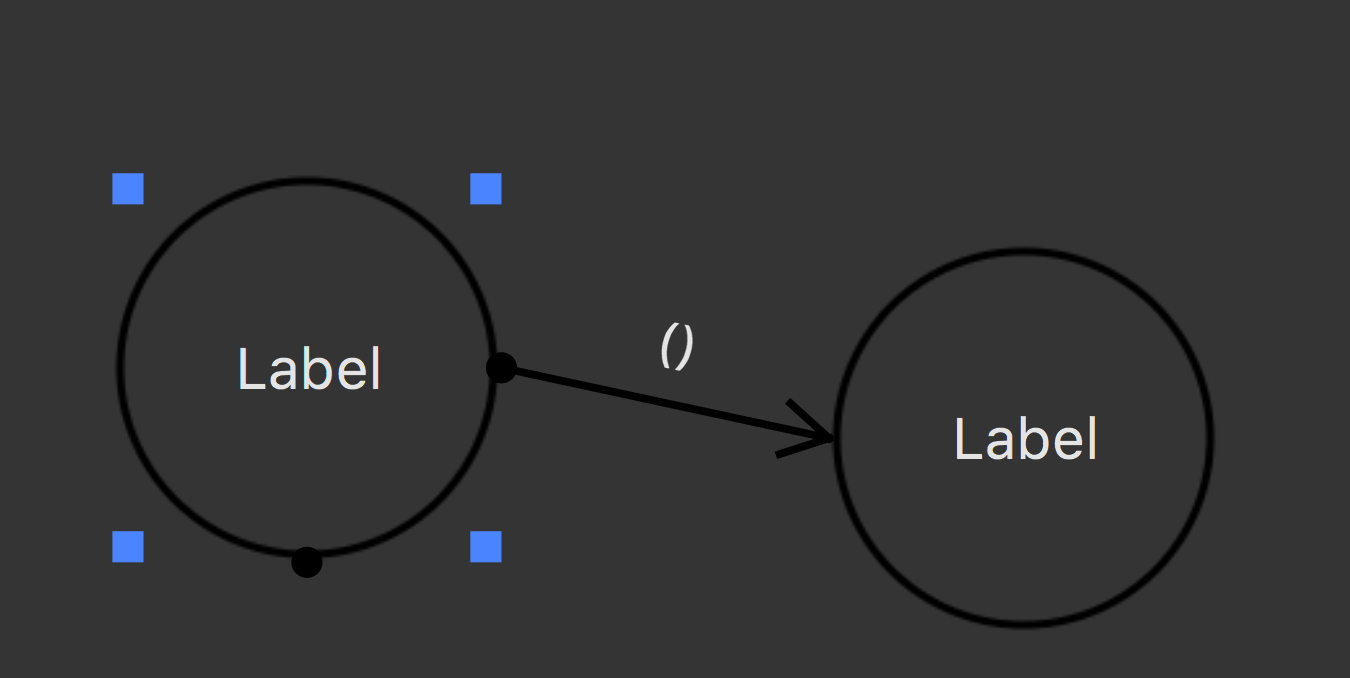
\includegraphics[width=.4\textwidth]{Zeichenflaeche_Basics2.png}
	\caption{Zeichenfläche - Erstellen einer Verbindung II}	
\end{figure}
Die Verbindung ist nun erstellt. Über dem Verbindungspfeil lässt sich hier nun ein Datenfluss eintragen. Dazu wählen Sie die Klammer aus und tragen die gewünschten Datentypen ein. 

\begin{figure}[H]
	\centering
	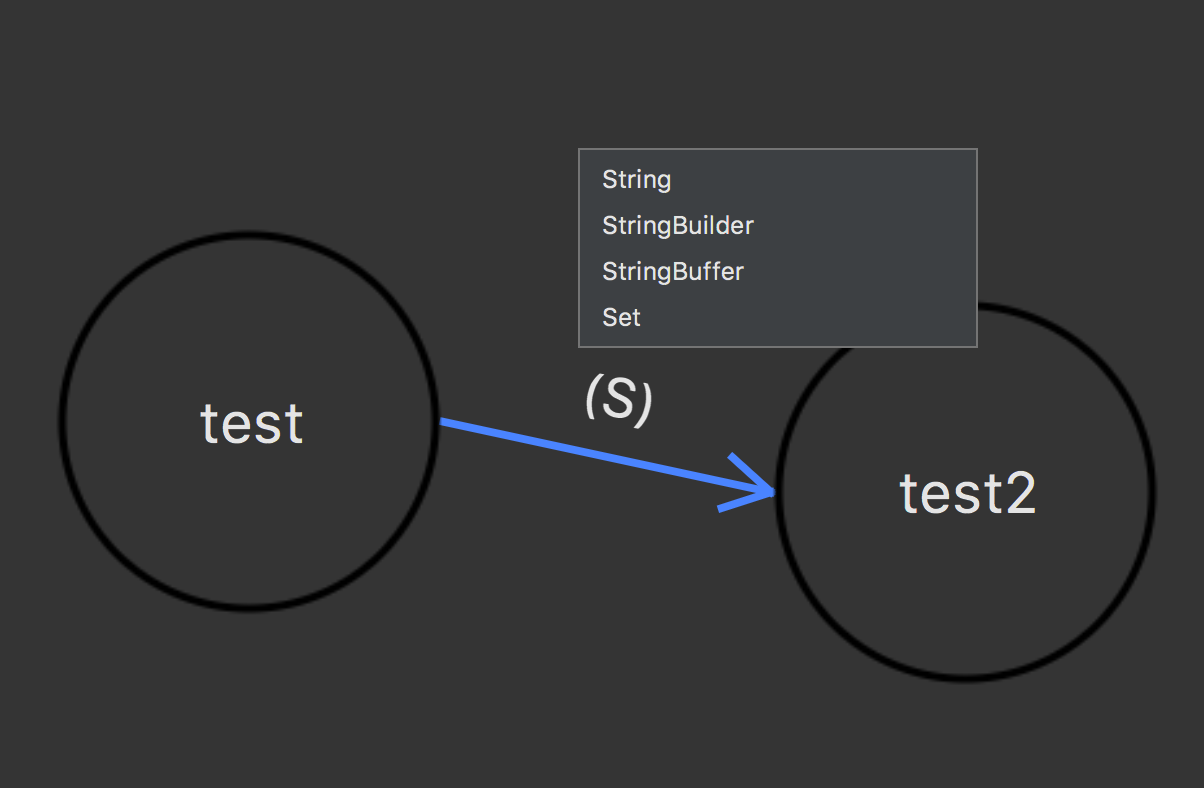
\includegraphics[width=.4\textwidth]{Zeichenflaeche_Basics3.png}
	\caption{Zeichenfläche - Erstellen einer Verbindung III}	
\end{figure}
Die Eingabe wird Ihnen durch eine automatische Autovervollständigung erleichtert. Es reicht den Anfangsbuchstaben des Datentyps anzugeben um eine Liste aller Typen mit jenen Buchstaben zu erhalten, welche sich in der Datentypenliste befinden. Nutzen Sie die Pfeiltasten zu Auswahl und bestätigen Sie mit Enter. Alternativ geben Sie den Typ manuell an.

\begin{figure}[H]
	\centering
	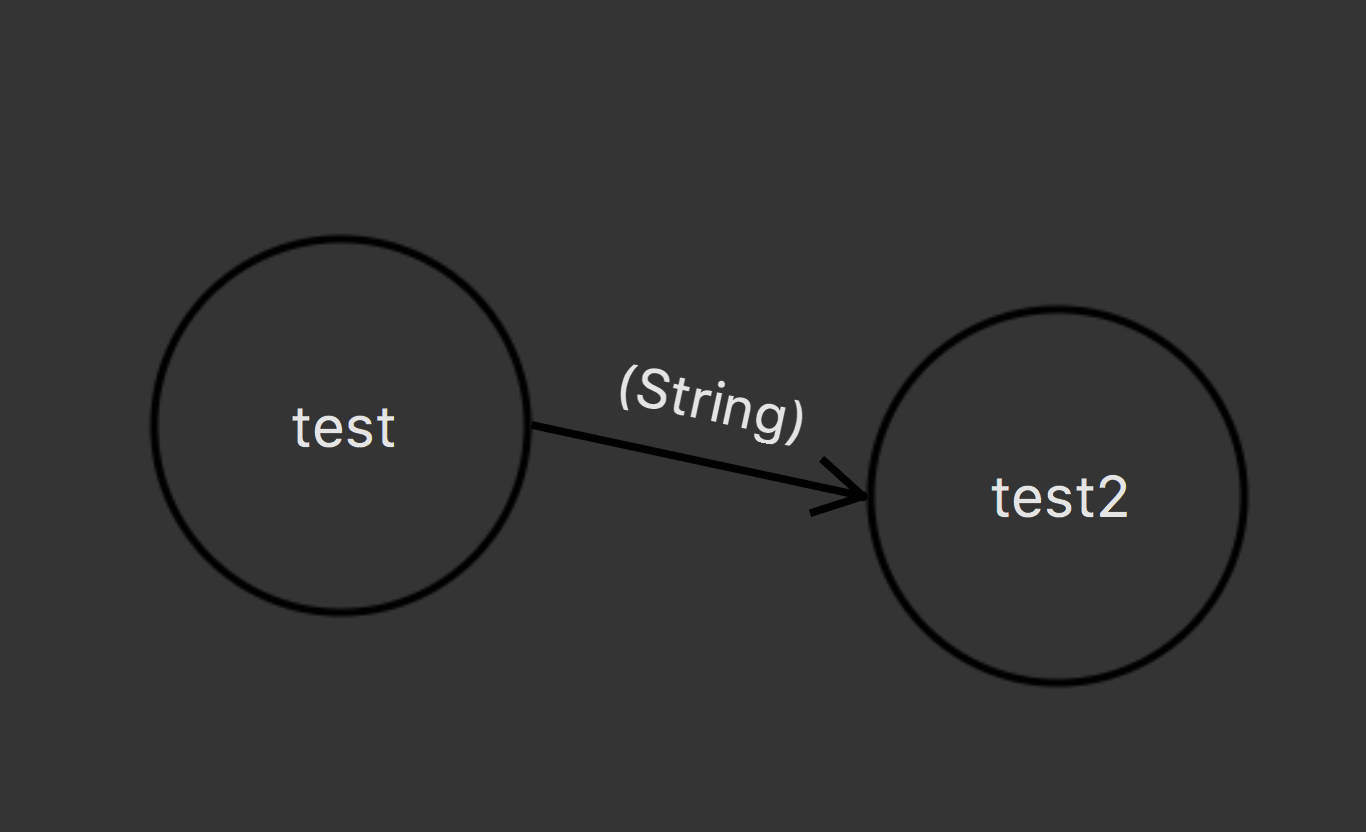
\includegraphics[width=.4\textwidth]{Zeichenflaeche_Basics4.png}
	\caption{Zeichenfläche - Erstellen einer Verbindung IV}	
\end{figure}
Sie sehen eine vollständige Verbindung mit Datenfluss. Mit einem Doppelklick auf das Element können Sie dieses ebenfalls umbenennen.

Um die Zeichenfläche nun zu verschieben, halten Sie die rechte Maustaste gedrückt und bewegen Sie die Maus. Zum Zoomen halten Sie Shift gedrückt und nutzen das Mausrad oder Touchpad.

\begin{figure}[H]
\subsubsection{Fortgeschrittene Programmfunktionen}
	\centering
	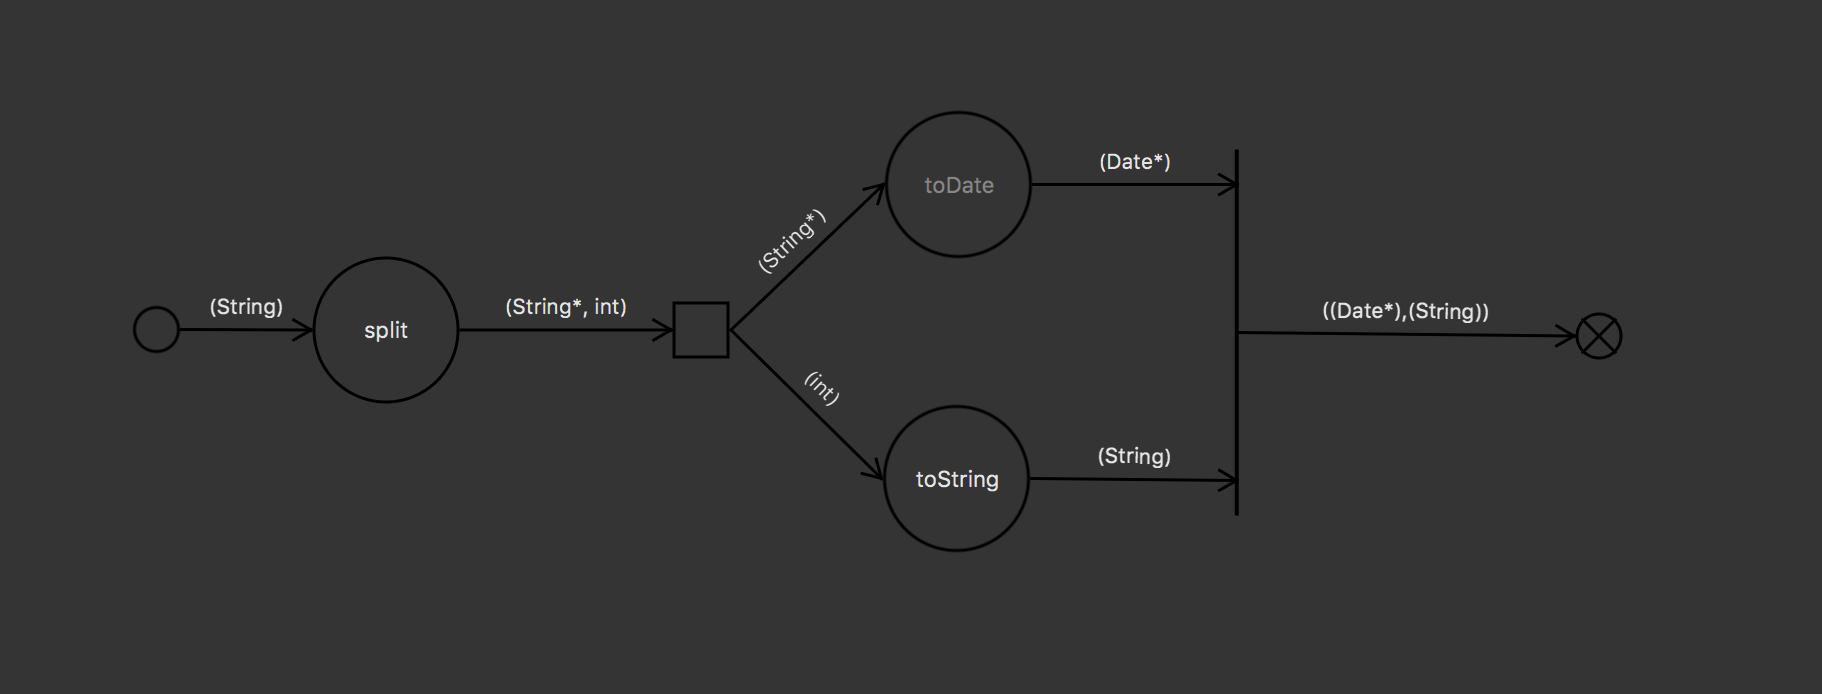
\includegraphics[width=1\textwidth]{Advanced.png}
	\caption{Zeichenfläche - Fortgeschrittene Funktionen}	
\end{figure}
Sie kennen nun bereits die grundlegenden Funktionen und Navigation. Bei einem vollständig modellierten Projekt sind folgende Funktionen besonders hilfreich:
\begin{itemize}
	\item Um in größeren Diagrammen schnell zwischen Elementen wechseln zu können, verwenden Sie die Tastenkombination Strg+Shift+Pfeiltaste rechts/links. 
	\item Wenn Sie, etwa eine Operation in einem Flow-Diagramm,  identisch zu einem Diagramm benennen, wird dieses automatisch referenziert. Dies erkennen Sie an der Grau-Färbung des Texts innerhalb des Elements.
\end{itemize}



\begin{figure}[H]
	\centering
	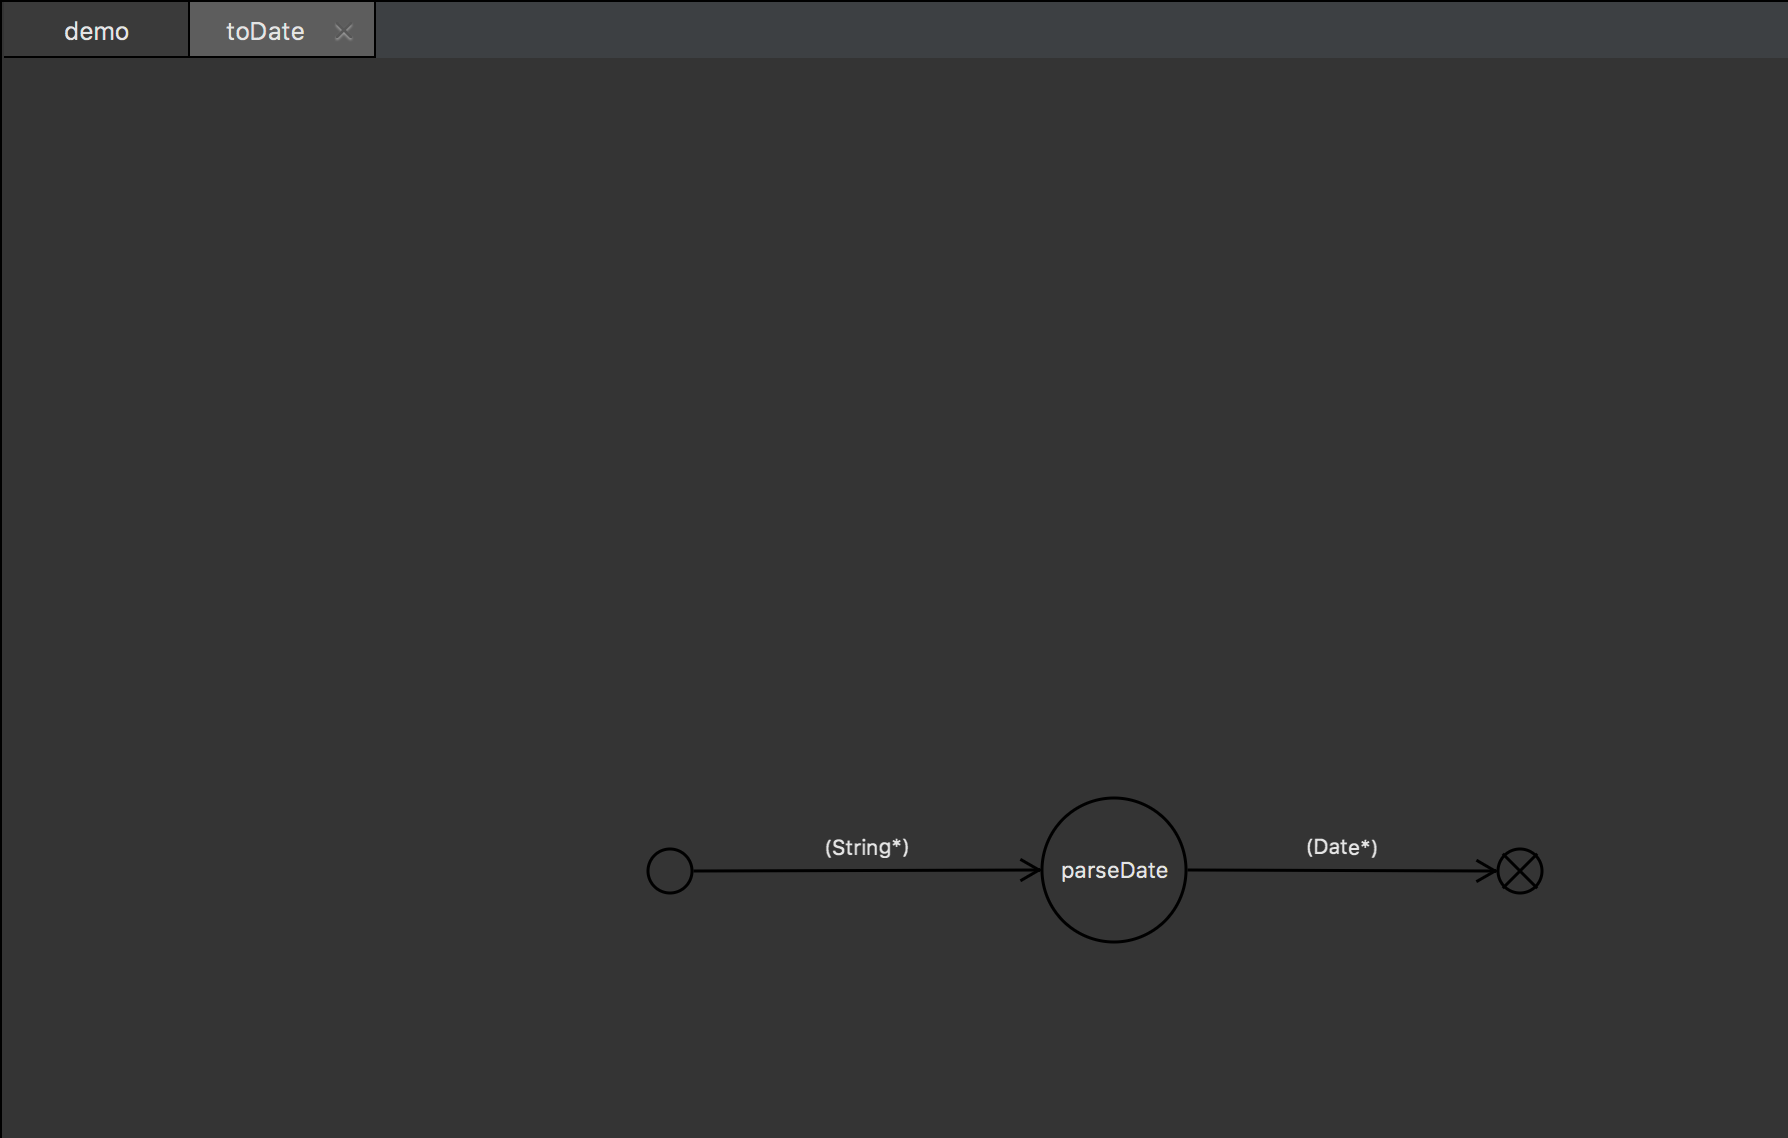
\includegraphics[width=1\textwidth]{Advanced2.png}
	\caption{Zeichenfläche - Fortgeschrittene Funktionen - Quick Jump}
\end{figure}
Nutzen Sie Strg+B nach der Auswahl eines referenzierten Elements um direkt in das dazugehörige Diagramm zu springen. In diesem Fall die Referenz der Operation ''toDate'' in das dazugehörige gleichnamige Diagramm.

\pagebreak
\begin{figure}[H]
	\centering
	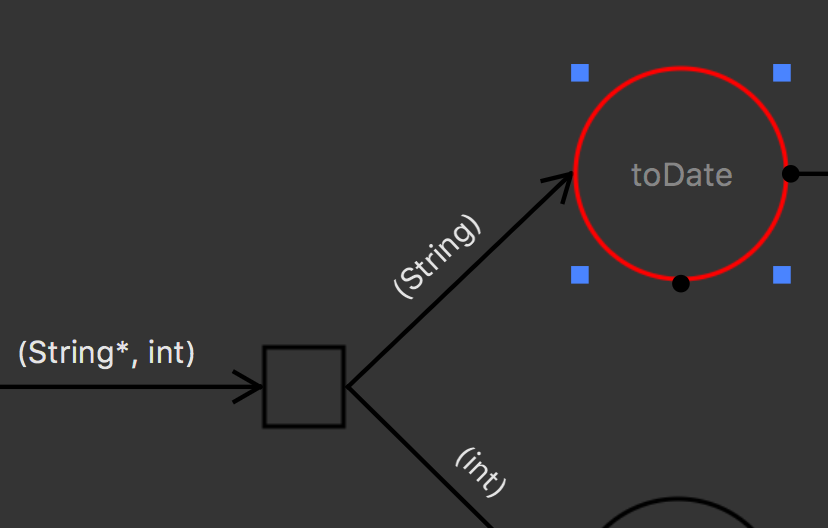
\includegraphics[width=.6\textwidth]{Advanced3.png}
	\caption{Zeichenfläche - Fortgeschrittene Funktionen - Eingabe/Ausgabe Typ}
\end{figure}

Das Programm überprüft, ob der Eingabe und Ausgabe Typ dem entspricht, was auch im referenzierten Diagramm hinterlegt ist.In diesem Beispiel erfordert ''toDate'' einen String-Pointer. Wird nur ein String übergeben, markiert sich das Element rot um auf einen Typemismatch aufmerksam zu machen. Wird der Fehler korrigiert oder die dahinter liegende Referenz angepasst, verschwindet der Fehler und damit auch die Färbung.

\begin{figure}[H]
	\centering
	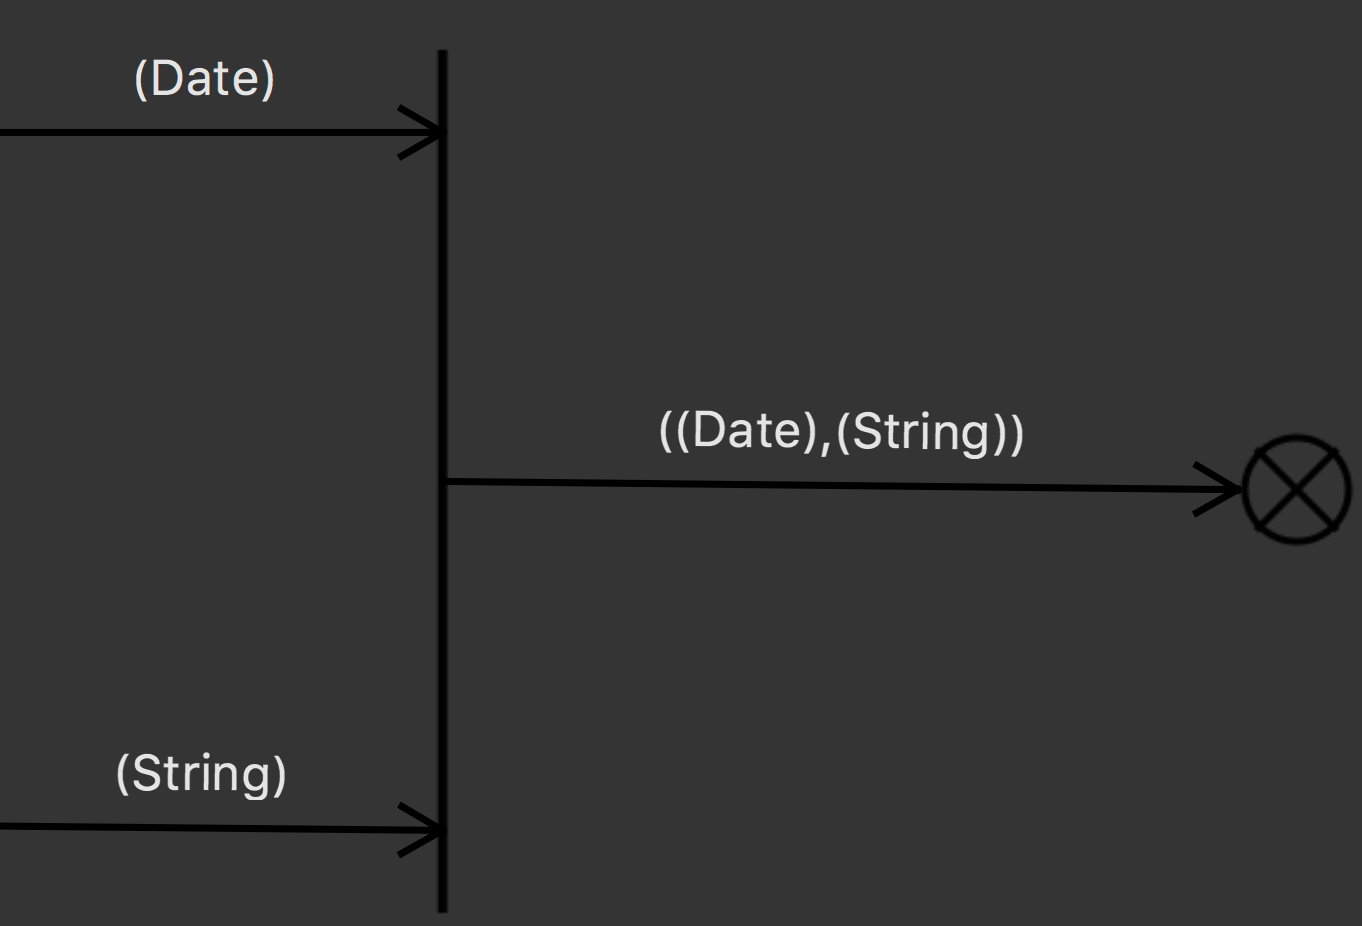
\includegraphics[width=.6\textwidth]{Quelle.png}
	\caption{Zeichenfläche - Fortgeschrittene Funktionen - Automatisches übernehmen}
\end{figure}
Falls Sie den Ausgabetyp einer Operation ändern und diese, wie etwa in diesem Beispiel, mit einer anderen zusammenläuft, haben Sie die Möglichkeit die Änderung automatisch durch das Programm übernehmen zu lassen. 

\begin{figure}[H]
	\centering
	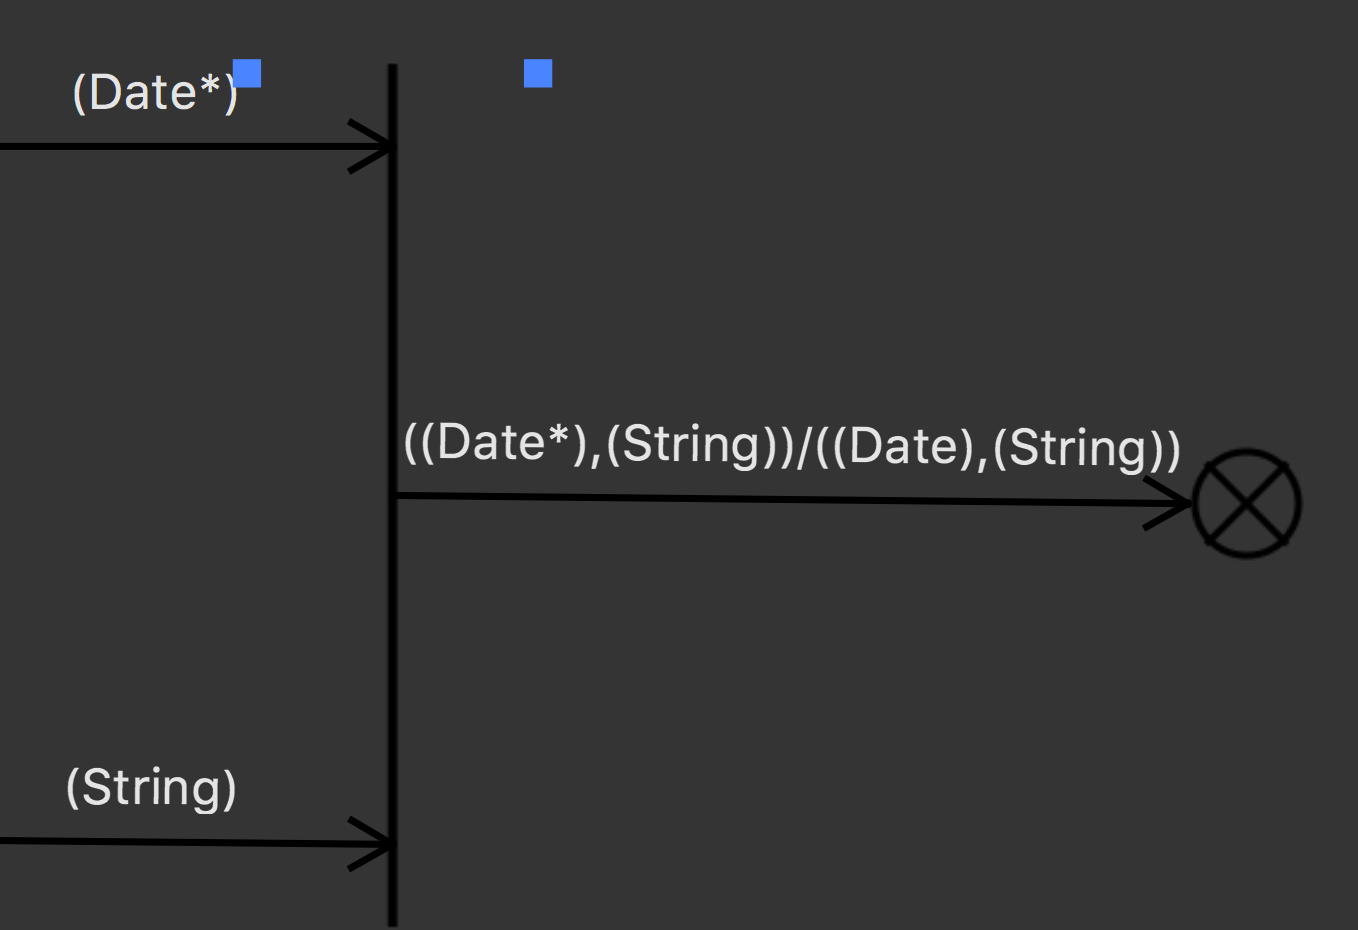
\includegraphics[width=.6\textwidth]{Quelle2.png}
	\caption{Zeichenfläche - Fortgeschrittene Funktionen - Automatisches übernehmen}
\end{figure}
''Date'' wurde hier nun zu ''Date*'' geändert. Das Programm zeig Ihnen bei der zusammenlaufenden Ausgabe nun den aktuellen und vorherigen Status an. 

\begin{figure}[H]
	\centering
	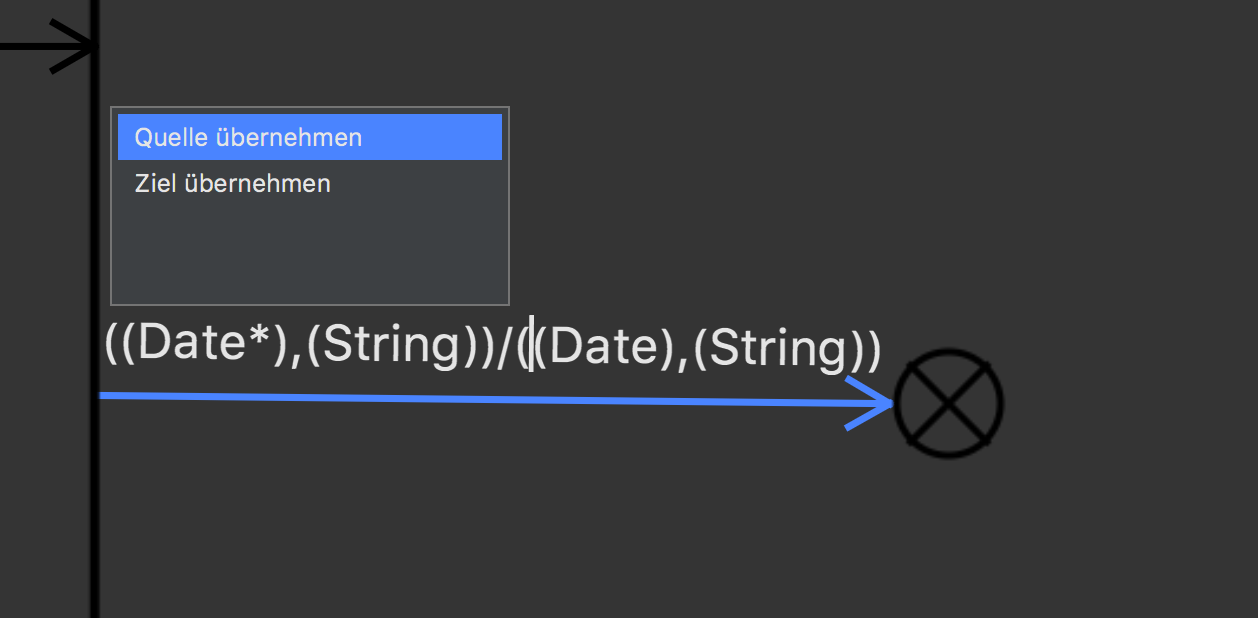
\includegraphics[width=.6\textwidth]{Quelle3.png}
	\caption{Zeichenfläche - Fortgeschrittene Funktionen - Automatisches übernehmen}
\end{figure}
Drücken Sie nun Strg+Alt+Enter nach Auswahl des gewünschten Feldes um das Kontextmenü aufzurufen. Wählen Sie ''Quelle übernehmen'' um automatisch die Änderung übernehmen zu lassen.

\begin{figure}[H]
	\centering
	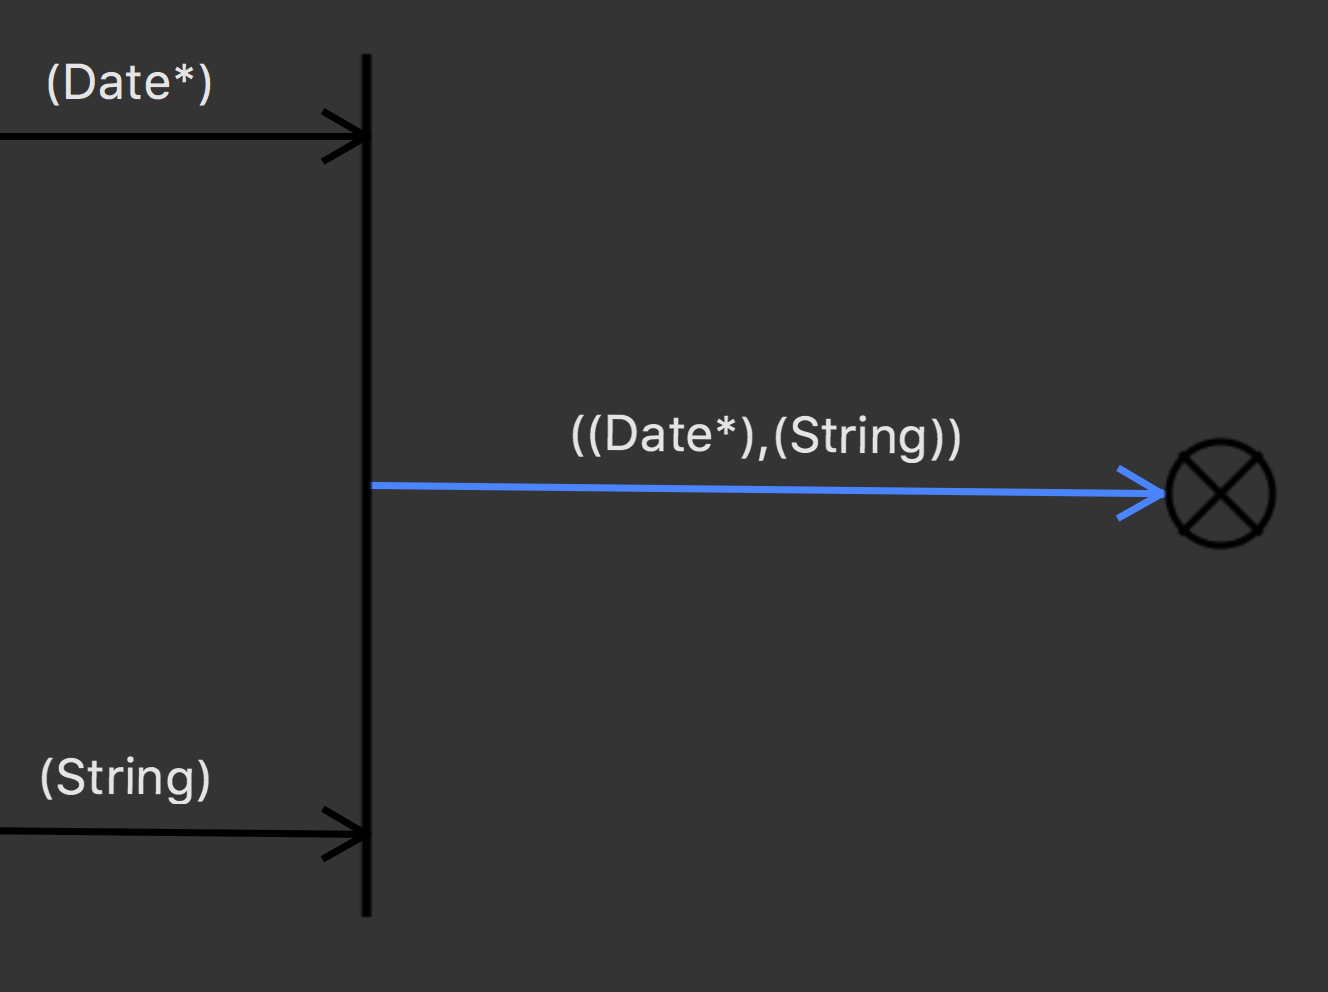
\includegraphics[width=.6\textwidth]{Quelle4.png}
	\caption{Zeichenfläche - Fortgeschrittene Funktionen - Automatisches übernehmen}
\end{figure}
Die Änderung wurde übernommen und die Typen stimmen jetzt mit der Änderung an der Quelle überein.

\pagebreak
\begin{figure}[H]
\subsubsection{Ändern des Programmdesigns und Suche}
	\centering
	
\includegraphics[width=.4\textwidth]{Design_Aendern.png}
	\caption{Designauswahl und Suche}
\end{figure}
Das Programm bietet Ihnen die Möglichkeit, zwischen drei verschiedenen Designs zu wählen. Zum Ändern des aktuellen Designs befindet sich im oberen rechten Teil des Fensters eine Designauswahl. Sie haben hier außerdem die Möglichkeit mit Hilfe des Lupensymbols die Suche aufzurufen (ebenfalls über die Menüleiste möglich, siehe 9.2.1).
\begin{figure}[H]
	\centering
	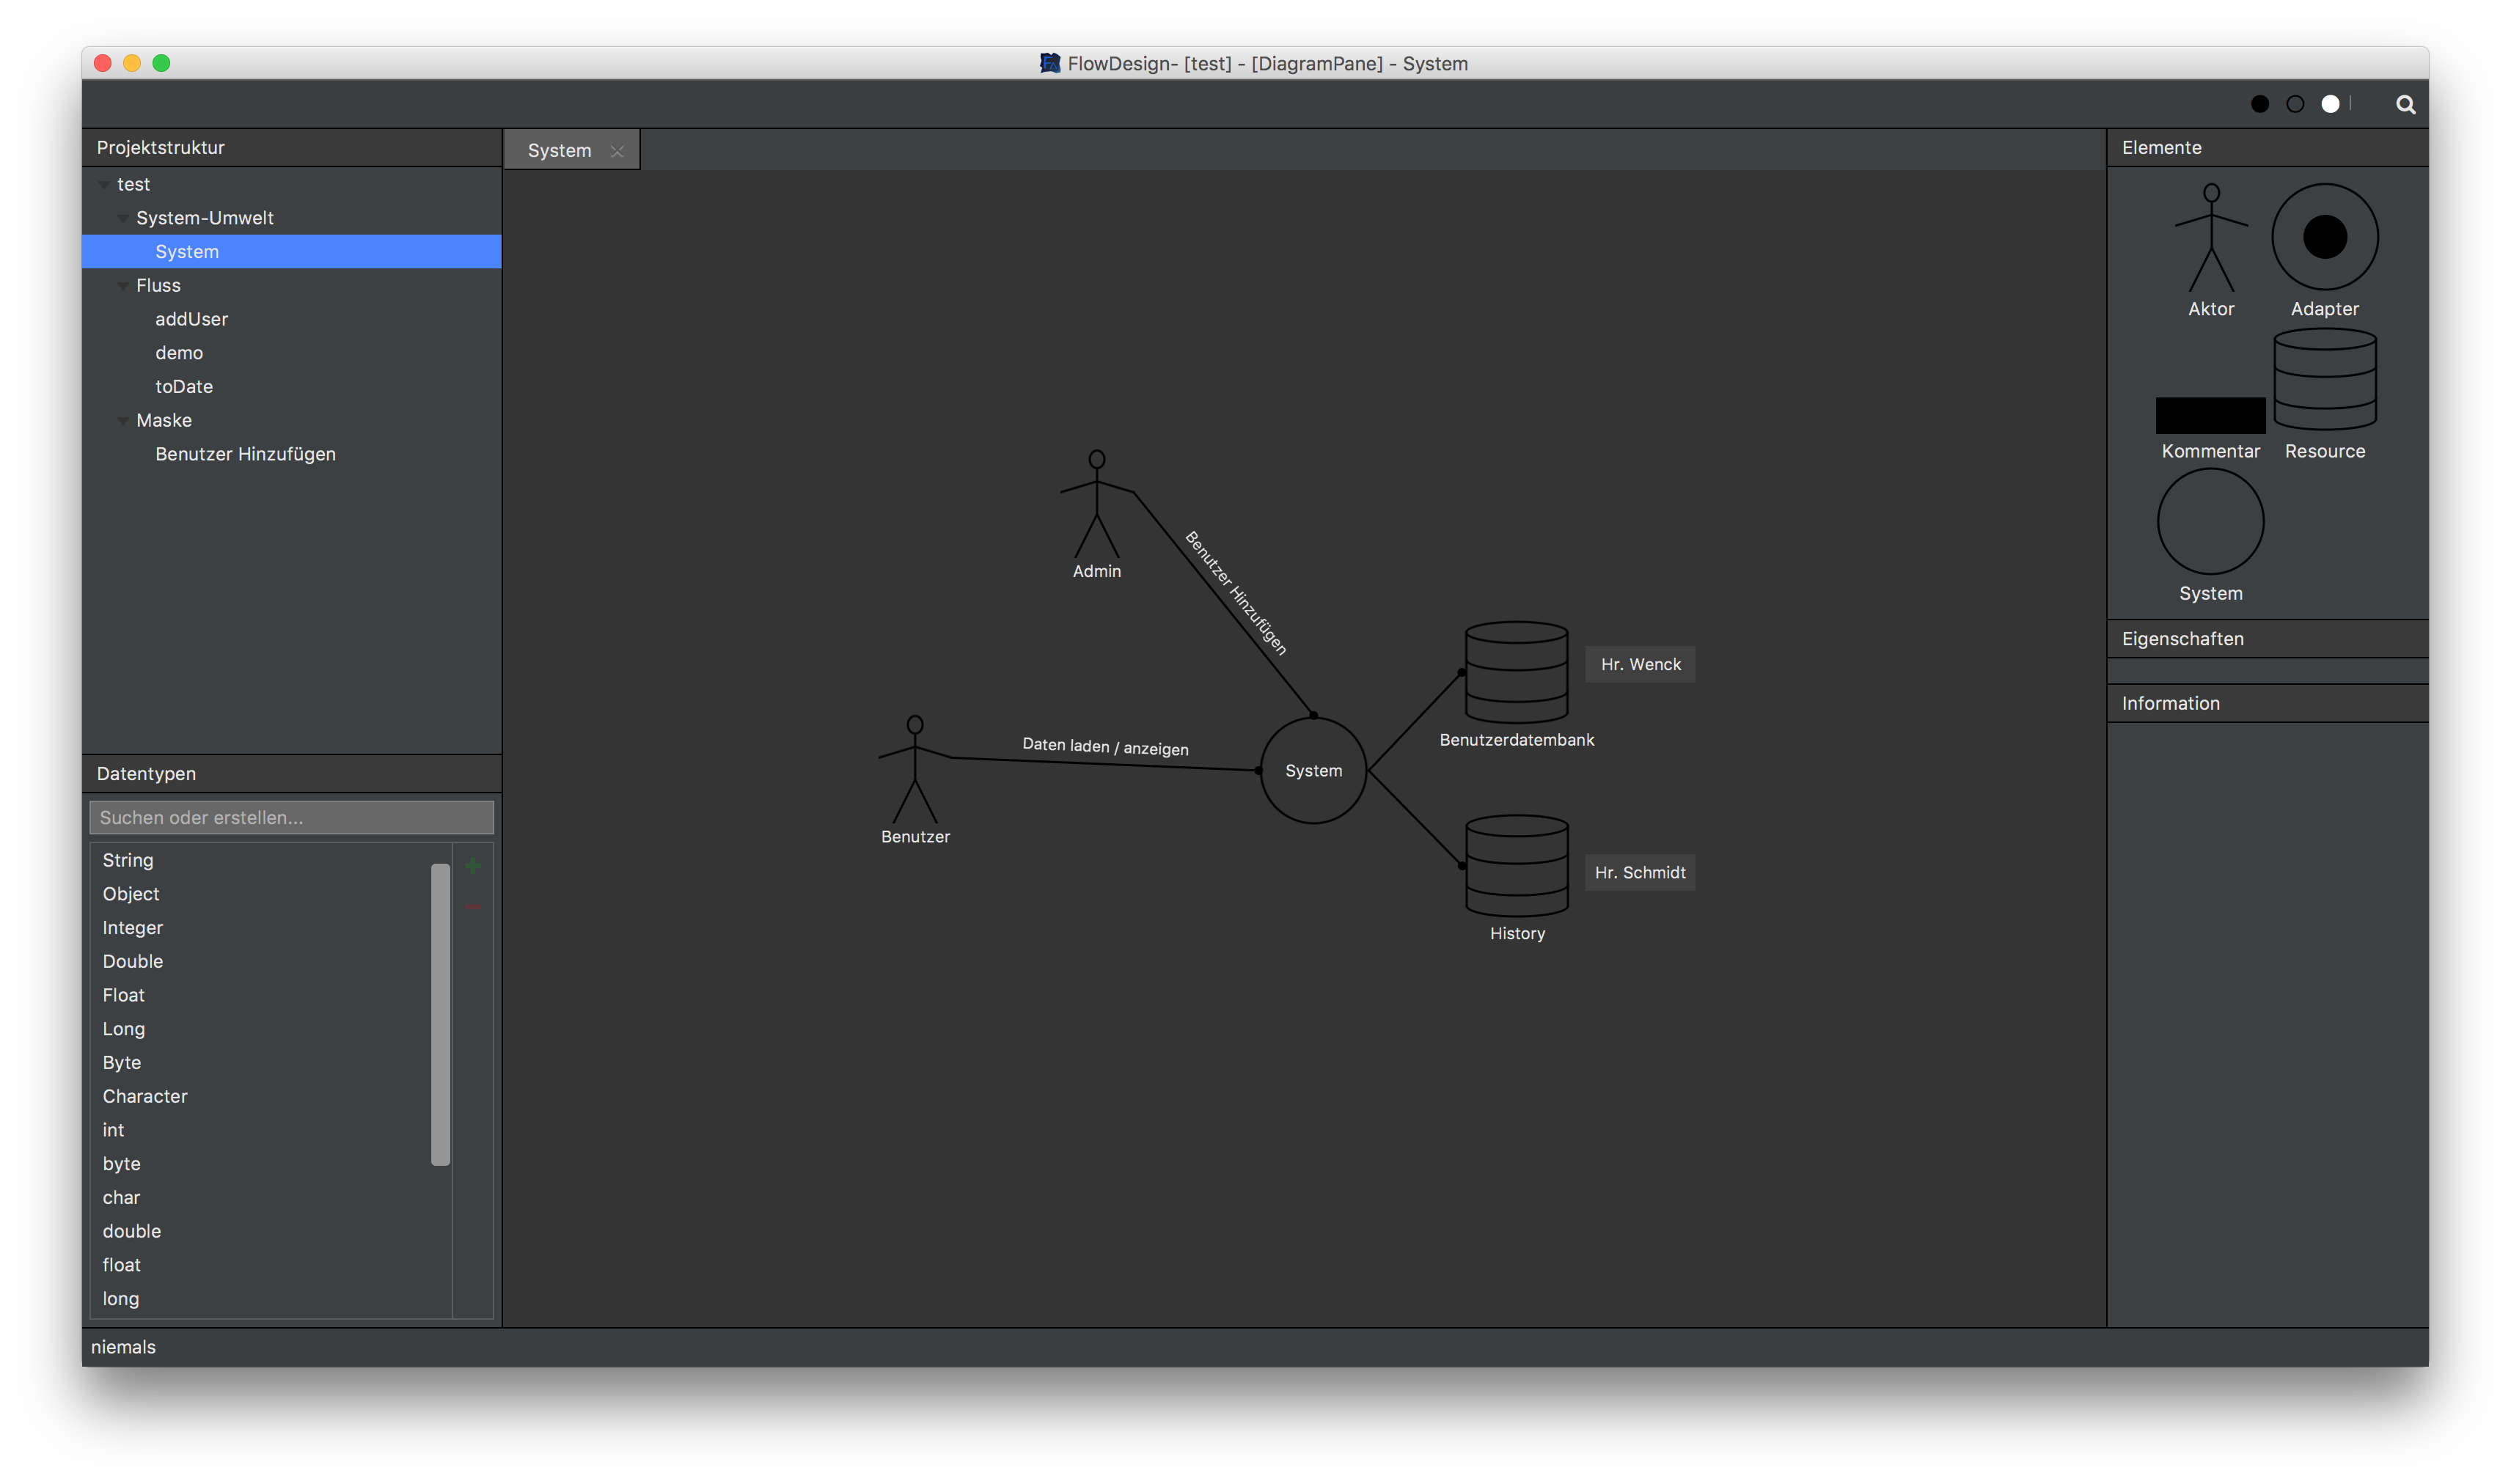
\includegraphics[width=.45\textwidth]{Design_Dark.png}
	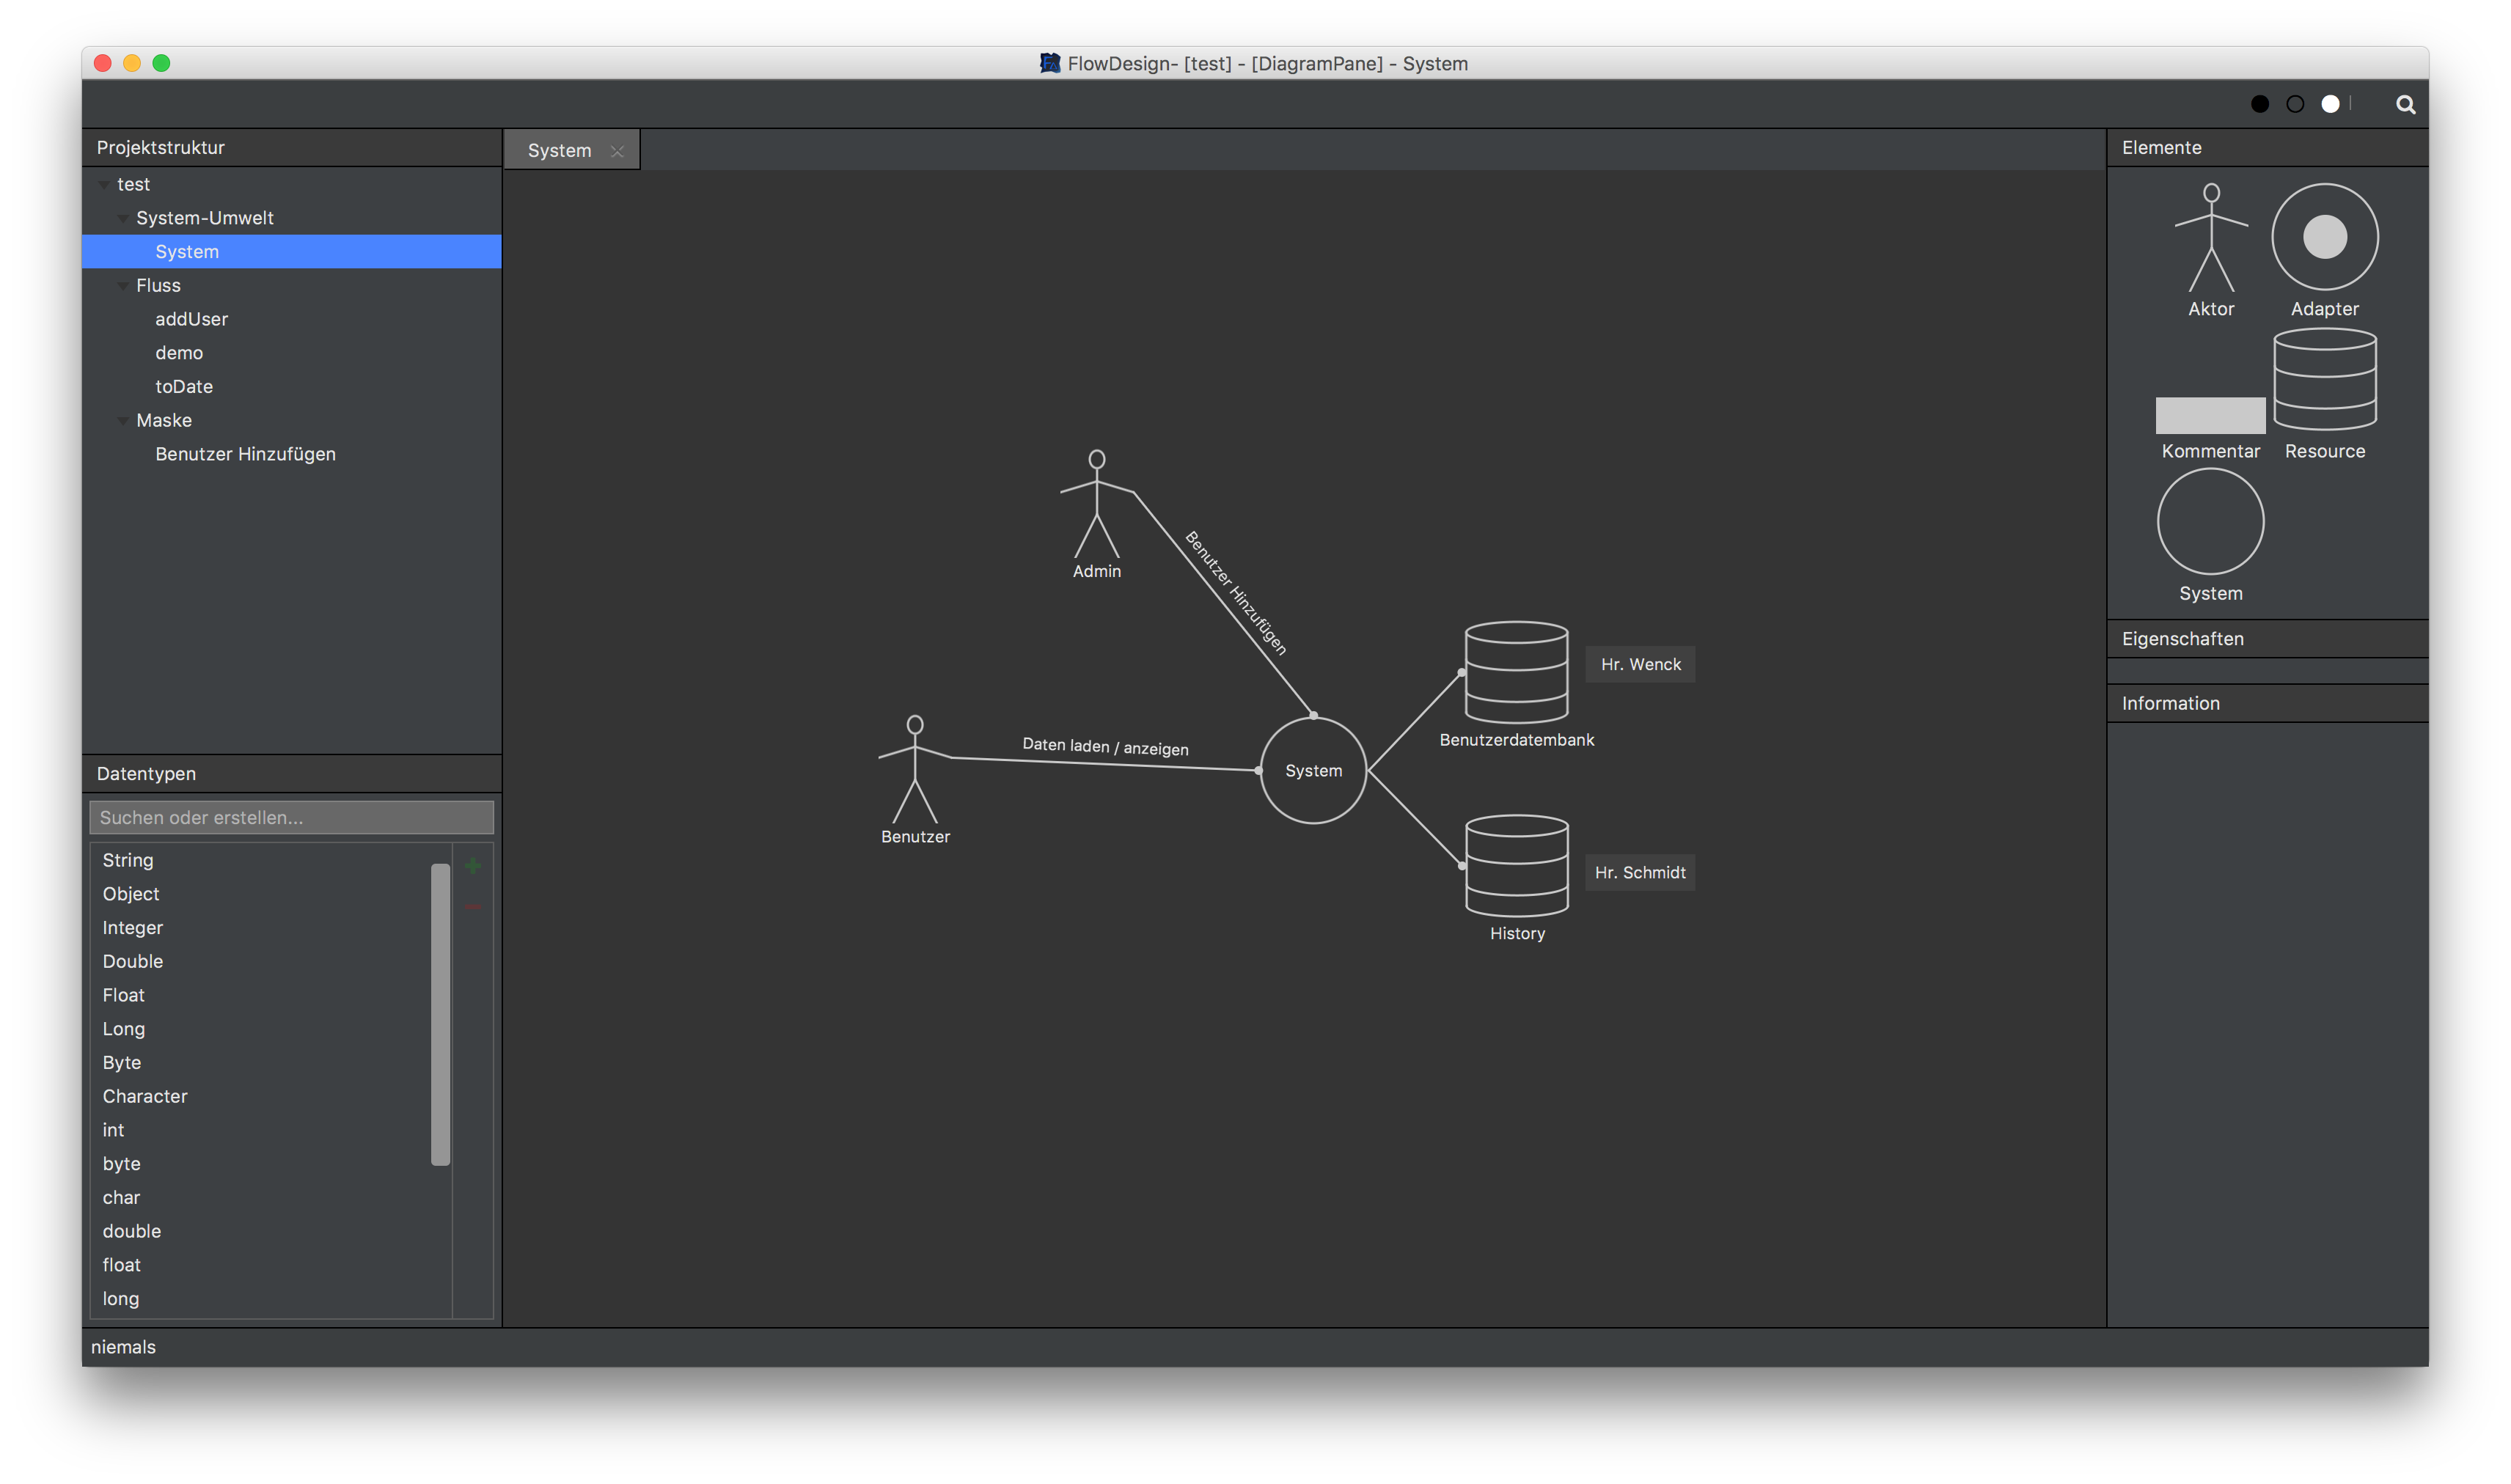
\includegraphics[width=.45\textwidth]{Design_Medium.png}
	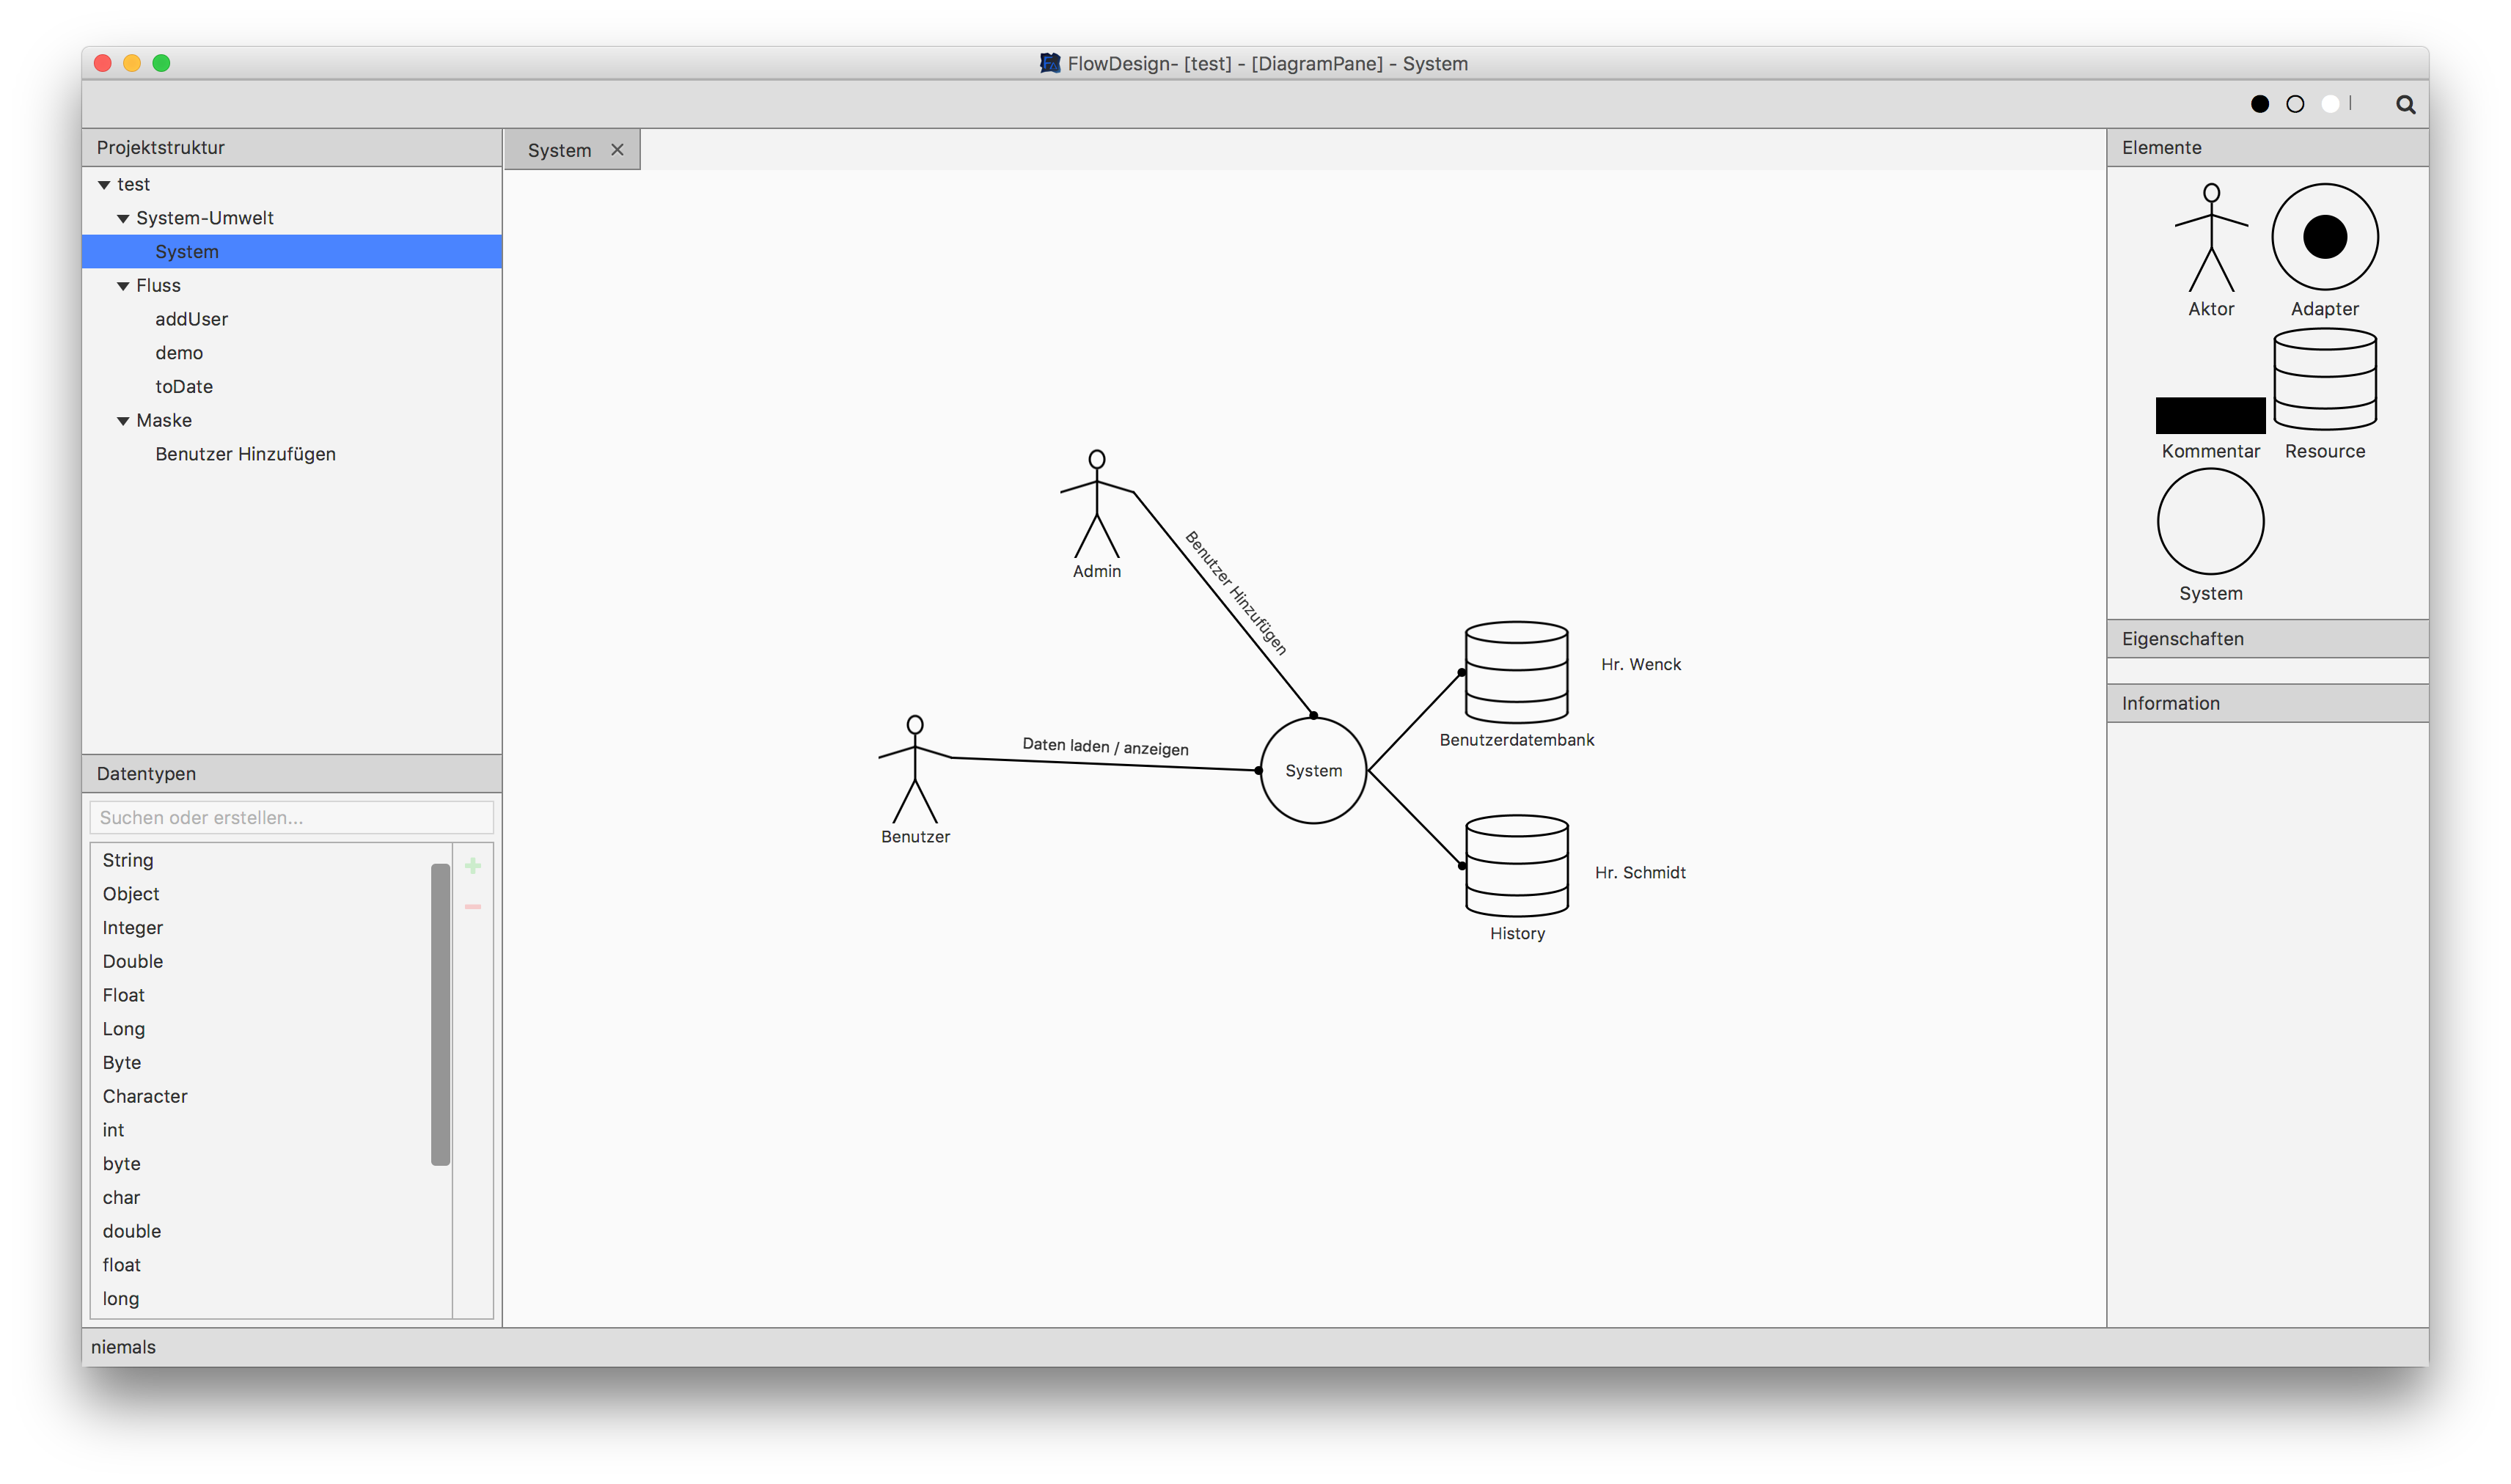
\includegraphics[width=.45\textwidth]{Design_Bright.png}
	\caption{Design - Dark, Medium, Bright}
\end{figure}

\begin{figure}[H]
	\centering
	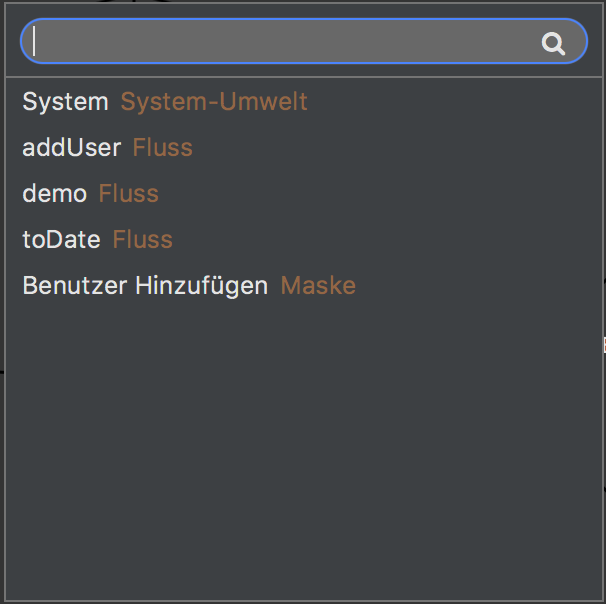
\includegraphics[width=.45\textwidth]{Search.png}
	\caption{Suchfenster}
\end{figure}
Nach betätigen des Lupensymbols erscheint ein Suchfenster. Es zeigt alle aktuell verfügbaren Diagramme innerhalb Ihres Projekts an. Dabei ist der Name eines Diagramms weiß und dessen Typ orange hervorgehoben. Sie können nun nach einem beliebigen Diagramm suchen, nutzen Sie dabei die Pfeiltasten zur Auswahl und bestätigen Sie mit Enter um direkt in das Diagramm zu gelangen.
